\subsection{微分形式，外微分}

回顾一下，在本篇以及后续各篇中，我们假定 K 的特征为 0，或者所考虑的簇在局部具有有限维。

8.3.1. 设 X 是 \(\mathbf{C}^r\) 类流形，且 F 是以 X 为基底的 \(\mathbf{C}^k\) 类向量丛，其中 \(k + 1 \in \mathbb{N}_{\mathbb{K}}\) 且 \(k + 1 \leqslant r\)。设 \(p\) 是一个 \(\geqslant 0\) 的整数，并令 \(\operatorname{Alt}^p(\mathrm{T}(\mathrm{X}); \mathrm{F})\) 为一个 \(\mathbf{C}^k\) 类向量丛，它由 \(p\)-交错多线性映射（从 \(\mathrm{T}(\mathrm{X})\) 到 F）组成（7.8.1 及第 7.8 号勘误）。X 的开集 U 上的这个丛的一个截面称为 U 上取值于 F、次数为 \(p\) 的交错微分形式（或简称微分形式）。属于 \(\mathbf{C}^k\) 类的这些截面构成一个 \(\mathcal{C}^k(\mathrm{U})\)-模，记为 \(^k\Omega^p(\mathrm{U}; \mathrm{F})\)。若 E 是 Banach 空间，则记 \(^k\Omega^p(\mathrm{U}; \mathrm{E})\) 而不记 \(^k\Omega^p(\mathrm{U}; \mathrm{E}_{\mathrm{x}})\)，并称为取值于 E 的微分形式。在这些记号中，有时省略 \(k\)（分别为 E），当它等于 \(r - 1\)（分别为 K）时。

取标量值的 0 次（分别为 1 次）微分形式是函数（分别是协向量场）。

设 \(\varphi\colon\mathbf{Y}\to\mathbf{X}\) 是 \(\mathbf{C}^{r}\) 类流形的态射，且 \(\omega\in{}^{k}\Omega^{p}(\mathbf{X};\mathbf{F})\)。则存在且仅存在一个形式 \(\varphi^{*}\omega\in{}^{k}\Omega^{p}(\mathbf{Y};\varphi^{*}\mathbf{F})\)，使得

\[
(\varphi^ {*} \omega) _ {y} (v _ {1}, \dots , v _ {p}) = \omega_ {\varphi (y)} (\mathrm{T} _ {y} (\varphi). v _ {1}, \dots , \mathrm{T} _ {y} (\varphi). v _ {p})\tag{1}
\]

对所有 \(y \in Y\) 以及 \(v_{1}, \ldots, v_{p}\) 中元素的任意族 \(\mathrm{T}_{y}(\mathrm{Y})\) 都成立。

若 \(\psi: Z \to Y\) 是 \(C^r\) 类流形的态射，则有

\[
(\varphi \circ \psi) ^ {*} \omega = \psi^ {*} (\varphi^ {*} \omega).\tag{2}
\]

当 Y 是 X 的子流形且 \(\varphi\) 是典范嵌入时，有时用 \(\omega|Y\) 代替 \(\varphi^{*}\omega\)，并称 \(\omega|Y\) 是由 \(\omega\) 在 Y 上诱导的形式。

8.3.2. 第 7.8 号的定义和结果适用于微分形式。特别地，向量丛的一个配对 \(F' \times_{\mathbf{X}} F'' \to F\) 产生一个外积 \(^k\Omega^{p'}(\mathrm{U};\mathrm{F}') \times ^k\Omega^{p''}(\mathrm{U};\mathrm{F}'') \to ^k\Omega^p(\mathrm{U};\mathrm{F})\)，其中 \(p = p' + p''\)（7.8.2）；记作 \((\omega', \omega'') \mapsto \omega' \wedge \omega''\)。因此，对所有 \(^k\Omega^p(\mathrm{U};\mathrm{K})\) 的 \(p \geqslant 0\) 的直和带有结合且交错的分次代数结构（A, III, p. 53）。

设 \(\xi\) 是 X 上的向量场，\(\omega\) 是 X 上取值于向量丛 F、次数为 \(p \geqslant 1\) 的微分形式；\(\xi\) 与 \(\omega\) 的内积是 X 上取值于 F、次数为 \(i(\xi, \omega)\) 的微分形式 \(p - 1\)，定义为

\[
i (\xi , \omega) _ {x} (v _ {1}, \dots , v _ {p - 1}) = \omega_ {x} (\xi (x), v _ {1}, \dots , v _ {p - 1})\tag{3}
\]

对所有 \(x \in X\) 以及 \(v_{1}, \ldots, v_{p-1}\) 中元素的任意族 \(\mathrm{T}_{x}(\mathrm{X})\) 都成立。若 \(\omega\) 是 0 次微分形式，令 \(i(\xi, \omega) = 0\)。我们也写作 \(i(\xi)\omega\) 或 \(i_{\xi}\omega\)，以代替 \(i(\xi, \omega)\)。当 \(\mathrm{F} = \mathrm{K}_{\mathrm{X}}\) 时，上述定义与 7.8.4 的定义一致。

设 \(\mathbf{F}' \times_{\mathbf{x}} \mathbf{F}'' \to \mathbf{F}\) 是向量丛的一个配对。对于 \(\omega' \in {}^k \Omega^{p'}(\mathbf{U}; \mathbf{F}')\) 和 \(\omega'' \in {}^k \Omega^{p''}(\mathbf{U}; \mathbf{F}'')\)，有

\[
i (\xi) \left(\omega^ {\prime} \wedge \omega^ {\prime \prime}\right) = \left(i (\xi) \omega^ {\prime}\right) \wedge \omega^ {\prime \prime} + (- 1) ^ {p ^ {\prime}} \omega^ {\prime} \wedge i (\xi) \omega^ {\prime \prime}.\tag{4}
\]

8.3.3. 设 \((u^{1},\ldots,u^{n})\) 是 X 的开集 U 上的坐标系。\(\omega\) 中的每个元素 \({}^{k}\Omega^{p}(\mathrm{U};\mathrm{F})\) 都唯一地写成

\[
\omega = \sum_ {i _ {1} <   \dots <   i _ {p}} f _ {i _ {1}, \dots , i _ {p}}. d u ^ {i _ {1}} \wedge \dots \wedge d u ^ {i _ {p}}
\]

其中 \(f_{i_1,\ldots,i_p}\) 是 \(\mathbf{C}^k\) 上 \(\mathbf{F}\) 的 \(\mathbf{U}\) 类截面；在此公式中，符号 \(\wedge\) 所涉及的是典范配对 \(\mathbf{K}_{\mathbf{x}} \times_{\mathbf{x}} \mathbf{K}_{\mathbf{x}} \to \mathbf{K}_{\mathbf{x}}\)，而表示乘积的点号所涉及的是典范配对 \(\mathbf{F} \times_{\mathbf{x}} \mathbf{K}_{\mathbf{x}} \to \mathbf{F}\)。

8.3.4. 设 \(p\) 是一个 \(\geqslant 0\) 的整数，\(r\) 是 \(\mathbf{N}_{\kappa}\) 的一个元素。设 \(E\) 和 \(F\) 是 Banach 空间，\(U\) 是 \(E\) 的开子集，且 \(\alpha \in {}^r\Omega^p(U;F)\)。令 \(\tilde{\alpha} \in \mathcal{C}^r (U; \operatorname{Alt}^p(E;F))\) 为对应于 \(\alpha\) 的元素。若 \(x \in U\)，则 \(d_x\tilde{\alpha}\) 是 \(\tilde{\alpha}\) 在 \(x\) 处的微分（5.5.6），它属于 \(\mathcal{L}(E; \operatorname{Alt}^p(E;F))\)；若 \(t \in E\)，则 \((d_x\tilde{\alpha})(t) \in \operatorname{Alt}^p(E;F)\)；而若 \(t_1, \ldots, t_p\) 属于 \(E\)，则 \((d_x\tilde{\alpha})(t)(t_1, \ldots, t_p) \in F\)。存在且仅存在一个元素 \(d\alpha\)；它属于 \({}^{r-1}\Omega^{p+1}(U;F)\)，使得

\[
(d \alpha) _ {x} (t _ {0}, \dots , t _ {p}) = \sum_ {i = 0} ^ {p} (- 1) ^ {i} (d _ {x} \tilde {\alpha}) (t _ {i}) (t _ {0}, \dots , \hat {t} _ {i}, \dots , t _ {p}) ^ {(1)}\tag{5}
\]

对所有 \(x \in U\) 以及 E 中的 \(t_{0}, \ldots, t_{p}\) 都成立。

8.3.5. 设 \(p\) 是一个 \(\geqslant 0\) 的整数，\(r\) 是 \(\mathbf{N}_{\mathbf{K}}\) 的一个元素。设 \(X\) 是 \(\mathbf{C}^{r+1}\) 类流形，\(F\) 是 Banach 空间，且 \(\omega \in {}^r\Omega^p(X;F)\)。存在且仅存在一个微分形式 \(\pi \in {}^{r-1}\Omega^{p+1}(X;F)\)，使得对于每个坐标图 \(c = (U,\varphi,E)\)（它是 \(X\) 的坐标图），若 \(\omega_c\) 是 \(\varphi(U)\) 上满足 \(\omega|U = \varphi^*(\omega_c)\) 的微分形式，则 \(\pi_c = d\omega_c\)，其中 \(d\omega_c\) 由 8.3.4 的公式 (5) 定义。

微分形式 \(\pi\) 称为 \(\omega\) 的外微分，记为 \(d\omega\)。它具有下列性质：

\begin{enumerate}
\def\labelenumi{(\arabic{enumi})}
\setcounter{enumi}{5}
\item
  若 \(\psi: Y \to X\) 是 \(C^{r+1}\) 类簇的态射且 \(\omega \in {}^r\Omega^n(X; F)\)，则有 \(\psi^*(d\omega) = d(\psi^*\omega)\)；特别地，\(d\) 与限制到子流形的运算可交换。
\item
  当 \(p = 0\) 时，映射 \(d: ^r\Omega^0(\mathbf{X}; \mathbf{F}) \to {}^{r-1}\Omega^1(\mathbf{X}; \mathbf{F})\) 与 8.2.2 中定义的映射一致。
\item
  若 \(r \geqslant 2\) 且 \(\omega \in {}^r\Omega^p(\mathbf{X};\mathbf{F})\)，则有 \(d(d\omega) = 0\)。\(^{(2)}\)
\item
  对 Banach 空间的每个连续线性映射 \(u: \mathbf{F} \to \mathbf{F}'\)，对于 \(d(u(\omega)) = u(d(\omega))\)，都有 \(\omega \in {}^{r}\Omega^{p}(\mathbf{U}; \mathbf{F})\)。
\item
  对 Banach 空间的每个连续双线性映射 \(F' \times F'' \rightarrow F\)，都有
\end{enumerate}

\[
d \left(\omega^ {\prime} \wedge \omega^ {\prime \prime}\right) = \left(d \omega^ {\prime}\right) \wedge \omega^ {\prime \prime} + (- 1) ^ {p ^ {\prime}} \omega^ {\prime} \wedge d \omega^ {\prime \prime}
\]

对于 \(\omega' \in {}^r\Omega^{p'}(\mathbf{X}; \mathbf{F}')\) 和 \(\omega'' \in {}^r\Omega^{p''}(\mathbf{X}; \mathbf{F}'')\)。


8.3.6. 设 \((u^{1},\ldots ,u^{n})\) 是 U 中 X 的一个坐标系。令

\[
\omega = \sum_ {i _ {1} <   \dots <   i _ {p}} f _ {i _ {1}, \dots , i _ {p}}. d u ^ {i _ {1}} \wedge \dots \wedge d u ^ {i _ {p}}
\]

\(^{1}\) 符号 \^{} 表示应省略它上方的符号（参见~7.8.4）。

\(^{2}\) 若 \(\omega\in^{1}\Omega^{p}(X;F)\) 且 \(d\omega\in^{1}\Omega^{p+1}(X;F)\)，仍有 \(d(d\omega)=0\)。

是 U 上的微分形式（其中 \(f_{i_1,\ldots,i_p} \in \mathcal{C}^r(\mathrm{U};\mathrm{F})\)）。于是有

\[
d \omega = \sum_ {i _ {1} <   \dots <   i _ {p}} d f _ {i _ {1}, \dots , i _ {p}} \wedge d u ^ {i _ {1}} \wedge \dots \wedge d u ^ {i _ {p}}.\tag{11}
\]

8.3.7. 假设 K 的特征为零。设 \(\omega \in {}^r\Omega^p (\mathbf{X};\mathbf{F})\) 是一个次数 \(p\geqslant 1\) 的微分形式，满足 \(d\omega = 0\)。对于每个 \(x\in \mathbf{X}\)，存在 \(x\) 的一个开邻域 U 以及一个 \(\pi \in {}^r\Omega^{p - 1}(\mathrm{U};\mathrm{F})\) 中的微分形式，使得在 U 上 \(d\pi = \omega\)。

\subsection{无穷小变换}

设 \(r \in \mathbf{N}_{\kappa}\)，且 \(X\) 是 \(\mathbf{C}^{r+1}\) 类流形。

8.4.1. 设 \(\tau\) 是一个 \(C^r\) 类同构向量函子（7.6.6）。若 E 是 Banach 空间，记 \(\mathbf{GL}(\mathbf{E})\) 为由 E 的自同构组成的 \(\mathcal{L}(\mathbf{E};\mathbf{E})\) 的开子集。记 \(\tau_{\mathbf{E}}'\) 为态射 \(\mathrm{Id}_{\mathbf{E}}\) 在单位元 \(\tau\colon\mathbf{GL}(\mathbf{E})\to\mathbf{GL}(\tau(\mathbf{E}))\) 处的线性切映射；它是从 \(\mathcal{L}(\mathbf{E};\mathbf{E})\) 到 \(\mathcal{L}(\tau(\mathbf{E});\tau(\mathbf{E}))\) 的连续线性映射。

8.4.2. 设 E 是 Banach 空间，并令 \(F = \tau(E)\)。设 U 是 E 的开子集，\(\xi\) 是 U 上的 \(C^r\) 类向量场，\(\tilde{\xi} \colon U \to E\) 是相应的映射（通过将 T(U) 与 U \times E 等同而得到（8.1.1）），且 \(f \colon U \to F\) 是一个 \(C^r\) 类映射。对于 \(x \in U\)，按下式定义 F 中的元素 \((\theta_\xi.f)(x)\)：

\[
(\theta_ {\xi}. f) (x) = d _ {x} f (\tilde {\xi} (x)) - \tau_ {\mathrm{E}} ^ {\prime} (d _ {x} \tilde {\xi}) (f (x)).\tag{1}
\]

（注意，一方面，\(\tilde{\xi}(x) \in \mathbf{E}\) 且 \(d_x f \in \mathcal{L}(\mathbf{E}; \mathbf{F})\)，因而 \(d_x f(\xi(x)) \in \mathbf{F}\)；另一方面，\(d_x \tilde{\xi} \in \mathcal{L}(\mathbf{E}; \mathbf{E})\)，\(\tau_{\mathbf{E}}'(d_x \tilde{\xi}) \in \mathcal{L}(\mathbf{F}; \mathbf{F})\)，且 \(f(x) \in \mathbf{F}\)，因而 \(\tau_{\mathbf{E}}'(d_x \tilde{\xi})(f(x)) \in \mathbf{F}\)。函数 \(\theta_{\xi}.f: x \mapsto (\theta_{\xi}.f)(x)\) 在 U 中属于 \(\mathbf{C}^{r-1}\) 类。）

8.4.3. 令 F 表示向量丛 \(\tau(\mathrm{T}(\mathrm{X}))\)（7.6.2 和 7.6.6）。设 \(\xi\) 是 X 上的向量场，\(f\) 是 F 的截面，二者都属于 \(\mathbf{C}^r\) 类。设 \(x\) 是 X 的一点，并设坐标图 \(c = (\mathrm{U}, \varphi, \mathrm{E})\)，它是 X 在 \(x\) 处的坐标图。令 \(c' = (\mathrm{U}, \zeta_c, \mathrm{E})\) 为 T(X) 相应的向量坐标图（8.1.1），令 \(\tau(c') = (\mathrm{U}, \psi_c, \tau(\mathrm{E}))\) 为 F 相应的向量坐标图（7.6.2）。置 \(x_c = \varphi(x)\)；令 \(\xi_c\) 为从 \(\varphi(\mathrm{U})\) 到 E 的映射，使得 \(\zeta_c(\xi(u)) = (u, \xi_c(\varphi(u)))\)，并令 \(f_c\) 为从 \(\varphi(\mathrm{U})\) 到 \(\tau(\mathrm{E})\) 的映射，使得 \(\psi_c(f(u)) = (u, f_c(\varphi(u)))\) 对所有 \(u \in \mathrm{U}\) 成立。将 8.4.2 中定义的 \(a_c\)（即 \((\theta_{\xi_c}.f_c)(x_c)\)）看作 \(\tau(\mathrm{E})\) 中的元素。存在且仅存在一个元素 \(a\)，属于 \(\mathrm{F}_x\)，使得 \(\psi_c(a) = (x, a_c)\) 对 X 的每个坐标图 \(c\)（在 \(x\) 处）都成立。记此元素为 \((\theta_\xi.f)(x)\)。它只取决于 \(\xi\) 和 \(f\) 在 \(x\) 处的芽（甚至只取决于它们的一阶喷射（12.1.2））。

映射 \(\theta_{\xi}.f: x \mapsto (\theta_{\xi}.f)(x)\) 是 F 的 \(\mathbf{C}^{r-1}\) 类截面；它关于对 \((\xi, f)\) 是 K-双线性的。

8.4.4. 保持前述假设和记号。存在（7.6.4）一个向量丛态射 \(\tau'\)；从 \(\mathcal{L}(\mathrm{T}(\mathrm{X});\mathrm{T}(\mathrm{X}))\) 到 \(\mathcal{L}(\mathrm{F};\mathrm{F})\) 的这种态射仅有一个，使得对所有 \(x \in X\)，\(\tau'\) 在纤维 \(\mathcal{L}(T(X); T(X))_x = \mathcal{L}(T_x(X); T_x(X))\) 上的限制等于 \(\tau_{T(X)}'\)（8.4.1）。若 \(g\) 是 \(C^r\) 类函数，定义在 \(X\) 上且取值于 \(K\)，则有

\[
\theta_ {g \xi}. f = g \theta_ {\xi}. f - \tau^ {\prime} (d g \otimes \xi) (f)
\]

（在此公式中，将 \(dg \otimes \xi\) 视为 \(T'(X) \otimes T(X)\) 的截面，并将其视为 \(\mathcal{L}(T(X); T(X))\) 的截面；其像 \(\tau'(dg \otimes \xi)\) 是 \(\mathcal{L}(F; F)\) 的截面，并将 \(f\) 映为 \(F\) 的截面）。

8.4.5. 设 I 是包含 0 的 K 的开子集，U 是 X 的开子集，且 \(\varphi\) 是从 \(C^r\) 到 X 的 \(\mathbf{I} \times \mathbf{U}\) 类映射。对于 \((t, x) \in \mathbf{I} \times \mathbf{U}\)，记向量 \(\varepsilon_{t,x}\) 为 \((1, 0) \in \mathbf{K} \times \mathrm{T}_x(\mathbf{X}) = \mathrm{T}_{(t,x)}(\mathbf{I} \times \mathbf{U})\)。对于 \(t \in \mathbf{I}\)，记从 U 到 X 的映射 \(\varphi_t\)，其定义为 \(\varphi_t(x) = \varphi(t, x) (x \in \mathbf{U})\)。假定满足下列三个条件：

\begin{enumerate}
\def\labelenumi{\alph{enumi})}
\item
  \(\varphi_{0}\) 是从 U 到 X 的典范嵌入；
\item
  对所有 \(t \in \mathbf{I}\)，映射 \(\varphi_t\) 是从 \(\mathbf{C}^r\) 到 \(\mathbf{U}\) 的某个开子集的 \(\mathbf{X}\) 类流形同构；
\item
  丛 \((t, x) \mapsto T_{(t, x)}(\varphi)(\varepsilon_{t,x})\) 的截面 \(\varphi^*T(X)\) 属于 \(C^r\) 类。此外，置：
\end{enumerate}

\[
d) \xi (x) = \mathrm{T} _ {(0, x)} (\varphi) (\varepsilon_ {0, x}) \quad \text {for all} \quad x \in \mathrm{U}.
\]

映射 \(\xi\colon x\mapsto\xi(x)\) 是 U 上的 \(\mathbf{C}^{r}\) 类向量场。称其为 \(\varphi\) 的初始（或起始）场。

设 \(\tau\) 是一个 \(C^r\) 类同构向量函子；置 \(F = \tau(T(X))\)，并设 \(f\) 是 \(C^r\) 类的、取值于 \(F\) 且定义在 \(X\) 上的截面。对于 \(x \in U\) 和 \(t \in I\)，置 \(\varphi_t^* f(x) = \tau(T_x(\varphi_t)^{-1})(f(\varphi_t(x)))\)；它是 \(F_x\) 中的元素。映射 \(t \mapsto \varphi_t^* f(x)\) 是从 \(I\) 到 \(F_x\) 的 \(C^{r-1}\) 类映射，对所有 \(x \in U\) 都成立，且有

\[
\frac {d}{d t} \left(\varphi_ {t} ^ {*} f (x)\right) _ {t = 0} = \left(\theta_ {\xi}. f\right) (x) \quad \text {for all} \quad x \in \mathrm{U}.\tag{2}
\]

8.4.6. 给定 X 上的 \(\xi\) 类向量场 \(C^r\) 及 X 的一点 \(x_0\)，存在包含 0 的 K 的开区间 I、包含 \(x_0\) 的 X 的开集 U，以及一个 \(\varphi: I \times U \to X\) 类映射 \(C^r\)，满足 8.4.5 的条件 \(a\)、\(b)\) 和 \(c)\)，且 \(\varphi\) 的初始场是 \(\xi|U\) 在 U 上的限制 \(\xi\)。

8.4.7. 例。--- 设 F 是 Banach 空间，p 是一个 \(\geqslant0\) 的整数。若 V 是 Banach 空间，置 \(\alpha_{p}(\mathbf{V}) = \operatorname{Alt}^{p}(\mathbf{V}; \mathbf{F})\)；若 u 是 V 到 Banach 空间 \(V'\) 的同构，记由 u 通过结构传递得到的从 \(\alpha_{p}(u)\) 到 \(\alpha_{p}(\mathbf{V})\) 的同构为 \(\alpha_{p}(\mathbf{V}')\)。由此得到一个同构向量函子，记为 \(\alpha_{p}\)（7.8.1 及第 7.8 号勘误）。可将前述结果应用于它；有

\[
\alpha_ {p} (\mathrm{T} (\mathrm{X})) = \operatorname{Alt}^{p}(\mathrm{T} (\mathrm{X}); \mathrm{F}).
\]

\(\alpha_{p}(\mathrm{T}(\mathrm{X}))\) 的截面是 \(p\) 次、定义在 \(\mathbf{X}\) 上且取值于 \(\mathbf{F}\) 的微分形式；若 \(\omega\) 是这样的形式，且 \(\xi\) 是 \(\mathbf{X}\) 上的向量场，二者都属于 \(\mathbf{C}^{r}\) 类，则 \(\theta_{\xi}.\omega\) 是 \(p\) 次、定义在 \(\mathbf{X}\) 上、取值于 \(\mathbf{F}\) 且属于 \(\mathbf{C}^{r-1}\) 类的微分形式。有

\[
\theta_ {\xi}. \omega = d (i (\xi) \omega) + i (\xi) d \omega\tag{3}
\]

并且当 \(r \geqslant 2\) 时，

\[
\theta_ {\xi}. d \omega = d (\theta_ {\xi}. \omega).\tag{4}
\]

当 \(p=0\) 时，函子 \(\alpha_{p}\) 是由 F 定义的常值向量函子；丛 \(\alpha_{0}(\mathrm{T}(\mathrm{X}))\) 与平凡丛 \(\mathrm{F}_{\mathrm{x}}\) 等同，而该丛的截面与 X 上取值于 F 的函数等同。若 \(\xi\) 是 X 上的 \(\mathbf{C}^{r}\) 类向量场，且 \(f\in\mathcal{C}^{r}(\mathrm{X};\mathrm{F})\)，则有

\begin{enumerate}
\def\labelenumi{(\arabic{enumi})}
\setcounter{enumi}{4}
\tightlist
\item
  \[
  \theta_ {\xi}. f = \langle \xi , d f \rangle = D _ {\xi} (f) \quad \text{(8.2.3)};
  \]
\end{enumerate}

它是 \(\mathcal{C}^{r-1}(X;F)\) 中的元素。

8.4.8. 设 \(\tau\) 和 \(\tau_{1}\) 是两个同构向量函子。向量函子的一个态射 \(h\colon \tau_{1}\to \tau\) 定义了从 \(h\) 到 \(\tau_{1}(\mathrm{T}(\mathbf{X}))\) 的向量丛态射（仍记为 \(\tau (\mathrm{T}(\mathbf{X}))\)）（7.6.4），并将 \(f\) 的一个截面 \(\tau_{1}(\mathrm{T}(\mathbf{X}))\) 对应为 \(h(f)\) 的一个截面 \(\tau (\mathrm{T}(\mathbf{X}))\)。若 \(\xi\) 是 \(\mathbf{X}\) 上的向量场，且 \(f\) 和 \(\xi\) 属于 \(\mathbf{C}^r\) 类，则有 \(\theta_{\xi}.h(f) = h(\theta_{\xi}.f)\)。

更一般地，设 \(\tau\)、\(\tau_{1},\ldots,\tau_{d}\) 是同构向量函子，且 \(h\colon(\tau_{1},\ldots,\tau_{d})\to\tau\) 是一个 \(d\)-线性态射（7.6.4）。设 \(f_{i}\in\mathcal{S}_{\tau_{i}(\mathrm{T}(\mathrm{X}))}^{r}(\mathrm{X})\)（对 \(i=1,\ldots,d\)），且 \(\xi\) 是 X 上的 \(\mathbf{C}^{r}\) 类向量场。有

\[
\theta_ {\xi}. h (f _ {1}, \dots , f _ {d}) = \sum_ {1 \leqslant i \leqslant d} h (f _ {1}, \dots , f _ {i - 1}, \theta_ {\xi}. f _ {i}, f _ {i + 1}, \dots , f _ {d}).\tag{6}
\]

例如，若 \(f\) 是 \(\tau(\mathrm{T}(\mathrm{X}))\) 的截面，\(g\) 是 \(\mathrm{X}\) 上取值于 \(\mathrm{K}\) 的函数，且二者都属于 \(\mathbf{C}^r\) 类，则有

\[
\theta_ {\xi}. (g f) = (\theta_ {\xi}. g) f + g (\theta_ {\xi}. f).\tag{7}
\]

若 \(\omega_{1}\) 和 \(\omega_{2}\) 是两个分别取值于 Banach 空间 \(C^{r}\) 和 \(F_{1}\) 的 \(F_{2}\) 类微分形式，则有

\[
\theta_ {\xi}. (\omega_ {1} \wedge \omega_ {2}) = (\theta_ {\xi}. \omega_ {1}) \wedge \omega_ {2} + \omega_ {1} \wedge (\theta_ {\xi}. \omega_ {2}),\tag{8}
\]

这里的外积是相对于从 \(F_{1} \times F_{2}\) 到 Banach 空间 F 的连续双线性映射而言的。

8.4.9. 设 \(\tau\) 是反变的（8.2.7）、\(\mathbf{C}^r\) 类同构向量函子，\(\varphi: X \to Y\) 是 \(\mathbf{C}^{r+1}\) 类流形的态射，\(\xi\)（分别为 \(\eta\)）是定义在 \(\mathbf{C}^r\)（分别为 \(X\)）上的 \(Y\) 类向量场，且 \(\xi\) 通过 \(\varphi\) 与 \(\eta\) 相关（8.2.6）。对于每个 \(f\)（它是 \(\tau(T(Y))\) 的 \(\mathbf{C}^r\) 类截面），有

\[
\varphi^ {*} (\theta_ {\eta}. f) = \theta_ {\xi}. \varphi^ {*} f.
\]

\subsection{括号}

设 \(r \in N_{K}\)，且 X 是 \(C^{r+1}\) 类流形。

8.5.1. 应用第 8.4 号的定义，取 \(\tau\) 为恒等函子：对每个 Banach 空间 V，有 \(\tau(\mathbf{V}) = \mathbf{V}\)，对 Banach 空间的每个同构 \(\tau(u) = u\)，有 \(u\)。于是 \(\tau(\mathrm{T}(\mathbf{X})) = \mathrm{T}(\mathbf{X})\)。若 \(\xi\) 和 \(\eta\) 是 \(\mathbf{C}^r\) 上的两个 \(\mathbf{X}\) 类向量场，置

\[
[ \xi , \eta ] = \theta_ {\xi}. \eta ;\tag{1}
\]

它是 X 上的 \(C^{r-1}\) 类向量场，称为 \(\xi\) 和 \(\eta\) 的括号。

8.5.2. 映射 \((\xi, \eta) \mapsto [\xi, \eta]\) 是 K-双线性且交错的。若 \(f\) 和 \(g\) 是 \(\mathbf{C}^r\) 上取值于 \(\mathbf{X}\) 的 \(\mathbf{K}\) 类函数，则有：

\[
[ f \xi , g \eta ] = f g [ \xi , \eta ] + (f D _ {\xi} g) \eta - (g D _ {\eta} f) \xi .\tag{2}
\]

8.5.3. 设 F 是 Banach 空间。有

\[
\mathbf {D} _ {[ \xi , \eta ]} = \mathbf {D} _ {\xi} \circ \mathbf {D} _ {\eta} - \mathbf {D} _ {\eta} \circ \mathbf {D} _ {\xi}\tag{3}
\]

在从 \(\mathcal{C}^{r+1}(X;F)\) 到 \(\mathcal{C}^{r-1}(X;F)\) 的映射空间中成立。

若 \(r \geqslant 2\)，且 \(\zeta\) 是 X 上的第三个 \(C^r\) 类向量场，则有

\[
[ [ \xi , \eta ], \zeta ] = [ \xi , [ \eta , \zeta ] ] - [ \eta , [ \xi , \zeta ] ] ^ {(1)}\tag{4}
\]

或者也可写成

\[
[ \xi , [ \eta , \zeta ] ] + [ \eta , [ \zeta , \xi ] ] + [ \zeta , [ \xi , \eta ] ] = 0.
\]

更一般地，若 \(r \geqslant 2\) 且 \(\tau\) 是同构向量函子，则有

\[
\theta_ {[ \xi , \eta ]} = \theta_ {\xi} \circ \theta _ {\eta} - \theta _ {\eta} \circ \theta_ {\xi}\tag{5}
\]

在从 \(\mathcal{C}^{r+1}(\mathrm{X};\mathrm{F})\) 到 \(\mathcal{C}^{r-1}(\mathrm{X};\mathrm{F})\) 的映射空间中成立（其中 \(\mathrm{F} = \tau (\mathrm{T}(\mathrm{X}))\)）。

若 \(r \geqslant \infty\)，则 X 上的 \(C^r\) 类向量场关于该括号构成 K-李代数（LIE, I, § 1, no. 2）。

8.5.4. 设 E 是 Banach 空间，U 是 E 的开子集，\(\xi\) 和 \(\eta\) 是 U 上的两个 \(C^{r}\) 类向量场，并将它们与 \(\mathcal{C}^{r}(U;E)\) 中的元素等同。它们的括号由下式给出：

\[
[ \xi , \eta ] = \mathbf {D} _ {\xi} \eta - \mathbf {D} _ {\eta} \xi .\tag{6}
\]

8.5.5. 设 \((u^1, \ldots, u^n)\) 是 X 在开集 U 上的坐标系。设 \(\xi = \sum a^i \frac{\partial}{\partial u^i}\) 和 \(\eta = \sum b^i \frac{\partial}{\partial u^i}\) 是 U 上的两个 \(C^r\) 类向量场。置 \([\xi, \eta] = \sum c^i \frac{\partial}{\partial u^i}\)。有

\[
c ^ {i} = \sum_ {1 \leqslant j \leqslant n} \left(a ^ {j} \frac {\partial b ^ {i}}{\partial u ^ {j}} - b ^ {j} \frac {\partial a ^ {i}}{\partial u ^ {j}}\right).\tag{7}
\]

8.5.6. 设 \(\varphi: X \to Y\) 是 \(C^{r+1}\) 类流形的态射，\(\xi_1\) 和 \(\xi_2\) 是 X 上的两个向量场，\(\eta_{1}\) 和 \(\eta_{2}\) 是 Y 上的两个向量场，且它们都属于 \(C^r\) 类。若 \(\xi_{1}\) 和 \(\xi_{2}\) 分别与 \(\varphi\) 和 \(\eta_{1}\) 由 \(\eta_{2}\) 相关，则 \([\xi_{1}, \xi_{2}]\) 与 \(\varphi\) 由 \([\eta_{1}, \eta_{2}]\) 相关。

8.5.7. 设 \(\omega\) 是 X 上取值于 Banach 空间 F、属于 \(p\) 类且次数为 \(\mathbf{C}^r\) 的微分形式，\(\xi_0, \ldots, \xi_p\) 是 X 上的 \(\mathbf{C}^r\) 类向量场。有

\[
(\theta_ {\xi_ {0}}. \omega) (\xi_ {1}, \dots , \xi_ {p}) = D _ {\xi_ {0}} \omega (\xi_ {1}, \dots , \xi_ {p}) - \sum_ {i = 1} ^ {p} \omega (\xi_ {1}, \dots , [ \xi_ {0}, \xi_ {i} ], \dots , \xi_ {p})\tag{8}
\]

并且

\[
\begin{array}{l} d \omega (\xi_ {0}, \dots , \xi_ {p}) = \sum_ {i = 0} ^ {p} (- 1) ^ {i} D _ {\xi_ {i}} \omega (\xi_ {0}, \dots , \hat {\xi} _ {i}, \dots , \xi_ {p}) \\ \qquad + \sum_ {i <   j} (- 1) ^ {i + j} \omega ([ \xi_ {i}, \xi_ {j} ], \xi_ {0}, \dots , \hat {\xi} _ {i}, \dots , \hat {\xi} _ {j}, \dots , \xi_ {p}). \end{array}\tag{9}
\]

若 \(\xi\) 和 \(\eta\) 是 \(\mathbf{C}^r\) 类向量场，则有

\[
\theta_ {\xi} \circ i (\eta) - i (\eta) \circ \theta_ {\xi} = i ([ \xi , \eta ])\tag{10}
\]

在从 \(^{r}\Omega^{p}(\mathbf{X};\mathbf{F})\) 到 \(^{r-1}\Omega^{p-1}(\mathbf{X};\mathbf{F})\) 的映射空间中成立。

当 \(p = 1\) 时，公式 (9) 变为：

\[
d \omega (\xi , \eta) = D _ {\xi} \langle \eta , \omega \rangle - D _ {\eta} \langle \xi , \omega \rangle - \langle [ \xi , \eta ], \omega \rangle .\tag{11}
\]

\subsection{提升}

设 \(r \in \mathbf{N}_{\mathbb{K}}\)，且 \(g: \mathbf{X} \to \mathbf{Y}\) 是 \(\mathbf{C}^{r+1}\) 类流形的态射。

8.6.1. g 在 T(Y) 中的一个提升是映射 \(\psi: X \to T(Y)\)，使得图表

\pandocbounded{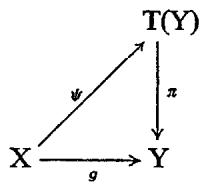
\includegraphics[keepaspectratio]{images/part001_bb2423ff.jpg}}

交换，其中 \(\pi\) 表示 T(Y) 到 Y 的典范投影。给定 \(\psi\) 等价于给定向量丛 \(g^{*}\mathrm{T}(\mathrm{Y})\) 的一个截面，即 T(Y) 在 g 下的逆像的一个截面。

提升的概念推广了向量场的概念（当 \(g = \operatorname{Id}_{\mathbf{X}}\) 时退化为向量场）；关于 \(\theta_{\xi}\) 和 \(i(\xi)\) 的定义与结果的重要部分也推广到提升；我们只简要指出其中几项。

8.6.2. 设 \(\psi: X \to T(Y)\) 是 \(g: X \to Y\) 的一个提升，并设 \(\omega\) 是一个 \(p\) 次、定义在 \(Y\) 上、取值于向量丛 \(F\)（其基底为 \(Y\)）的微分形式。当 \(p \geqslant 1\) 时，将微分形式 \(i(\psi,\omega)\)、或 \(i(\psi)\omega\)、或 \(i_{\psi}(\omega)\) 记在 X 上；它们的次数为 \(p-1\)，取值于 \(g^{*}\mathbf{F}\)，并满足

\[
i (\psi , \omega) _ {x} (v _ {1}, \dots , v _ {p - 1}) = \omega_ {g (x)} (\psi (x), T _ {x} (g). v _ {1}, \dots , T _ {x} (g). v _ {p - 1})\tag{1}
\]

对所有 \(x \in X\) 以及每个 \(v_1, \ldots, v_{p-1}\)（其元素属于 \(\mathbf{T}_x(X)\)），上述关系都成立。当 \(p = 0\) 时，令 \(i(\psi, \omega) = 0\)。称 \(i(\psi, \omega)\) 为 \(\psi\) 与 \(\omega\) 的内积；若 \(\psi\) 和 \(\omega\) 属于 \(\mathbf{C}^r\) 类，则 \(i(\psi, \omega)\) 也属于该类。设 \(\mathbf{F}' \times_{\mathbb{Y}} \mathbf{F}'' \to \mathbf{F}\) 是以 Y 为基底的向量丛的一个配对。对于 \(\omega' \in {}^\tau \Omega^{p'}(Y; F')\) 和 \(\omega'' \in {}^\tau \Omega^{p''}(Y; F'')\)，有

\[
i (\psi) \left(\omega^ {\prime} \wedge \omega^ {\prime \prime}\right) = (i (\psi) \omega^ {\prime}) \wedge g ^ {*} \omega^ {\prime \prime} + (- 1) ^ {p ^ {\prime}} g ^ {*} \omega^ {\prime} \wedge i (\psi) \omega^ {\prime \prime}.\tag{2}
\]

8.6.3. 例子

\begin{enumerate}
\def\labelenumi{\alph{enumi})}
\tightlist
\item
  X 上的向量场 \(\xi\) 定义了 g 在 T(Y) 中的提升 T(g) \(\circ\) \(\xi\)，并且有：
\end{enumerate}

\[
i (\mathrm{T} (g) \circ \xi) = i (\xi) \circ g ^ {*}.\tag{3}
\]

\begin{enumerate}
\def\labelenumi{\alph{enumi})}
\setcounter{enumi}{1}
\tightlist
\item
  Y 上的向量场 \(\eta\) 定义了 \(\eta \circ g\) 在 T(Y) 中的提升 \(g\)，并且有：
\end{enumerate}

\[
i (\eta \circ g) = g ^ {*} \circ i (\eta).\tag{4}
\]

\begin{enumerate}
\def\labelenumi{\alph{enumi})}
\setcounter{enumi}{2}
\tightlist
\item
  更一般地，设 \(h: \mathbf{Y} \to \mathbf{Z}\) 是 \(\mathbf{C}^{r+1}\) 类流形的态射。若 \(\psi\) 是 \(g\) 到 \(\mathbf{T}(\mathbf{Y})\) 的提升，则 \(\mathbf{T}(h) \circ \psi\) 是 \(h \circ g\) 到 \(\mathbf{T}(\mathbf{Z})\) 的提升，并且有：
\end{enumerate}

\[
i (\mathrm{T} (h) \circ \psi) = i (\psi) \circ h ^ {*}.\tag{5}
\]

若 \(\varphi\) 是 \(h\) 到 \(\mathrm{T}(Z)\) 的提升，则 \(\varphi \circ g\) 是 \(h \circ g\) 到 \(\mathrm{T}(Z)\) 的提升，并且有：

\[
i (\varphi \circ g) = g ^ {*} \circ i (\varphi).\tag{6}
\]

8.6.4（“无穷小变换”）。设 \(\psi\) 是 \(C^r\) 类的 \(g\) 的提升，且 \(\omega\) 是 Y 上取值于 Banach 空间 F、次数为 \(p\) 且属于 \(C^r\) 类的微分形式。X 上的微分形式

\[
d (i (\psi) \omega) + i (\psi) d \omega\tag{7}
\]

是次数为 \(p\) 的 \(\mathbf{C}^{r-1}\) 类形式；记为 \(\theta_{\psi}.\omega\)。

若 f 是 X 上的 \(C^{r}\) 类函数，则有

\[
\theta_ {f \psi}. \omega = d f \wedge i (\psi) \omega + f \theta_ {\psi}. \omega .\tag{8}
\]

8.6.5（“将 \(\theta_{\psi}.\omega\) 刻画为导数”）。保持 8.6.4 的假设。设 \(x\in X\)。则存在 \(x\) 的一个开邻域 U、K 中 0 的一个开邻域 I，以及一个 \(C^{r}\) 类态射 G: I × U → Y，具有下列两个性质：

\begin{enumerate}
\def\labelenumi{\alph{enumi})}
\item
  对每个 \(x \in \mathbf{U}\)，有 \(\mathbf{G}(0, x) = g(x)\)。
\item
  对每个 \(x \in \mathbf{U}\)，切向量 (1, 0) 在 \(\mathrm{T}_{(0,x)}(\mathrm{G})\) 下的像等于 \(\psi(x)\)。
\end{enumerate}

设 (U, I, G) 满足这些条件；对于每个 \(t \in \mathbf{I}\)，记从 U 到 Y 的映射 \(\mathbf{G}_t\) 为 \(x \mapsto \mathbf{G}(t, x)\)；置 \(\omega_t = \mathbf{G}_t^*(\omega)\)。对于每个 \(x \in \mathbf{X}\)，从 I 到 \(t \mapsto \omega_t(x)\) 的映射 \(\operatorname{Alt}^p(\mathrm{T}_x(\mathbf{X}), \mathbf{F})\) 属于 \(\mathbf{C}^r\) 类，且其在原点处的导数由下式给出

\[
\frac {d}{d t} (\omega_ {t} (x)) _ {t = 0} = (\theta_ {\psi}. \omega) (x).\tag{9}
\]

\subsection{结构的弱化}

本节假设 K = R。

8.7.1. 设 X 是 \(C^{s}\) 类流形，F 是 X 上的 \(C^{k}\) 类向量丛，其中 \(0 \leqslant k \leqslant s\)。若 \(0 \leqslant k' \leqslant k\)，则 F 上存在唯一的、以 X 为基底且属于 \(F_{k'}\) 类的向量丛结构 \(C^{k'}\)，使得 F 的每个向量坐标图都是 \(F_{k'}\) 的向量坐标图。称 \(F_{k'}\) 是通过弱化 F 的丛结构从 F 得到的。

8.7.2. 设 \(r \in \mathbf{N}_{\mathbb{R}}\) 且 \(r \leqslant s\)，令 \(\mathbf{X}_r\) 为以 \(\mathbf{C}^r\) 为底层的 \(\mathbf{X}\) 类流形（5.13.1）。切丛 \(\mathrm{T}(\mathbf{X}_r)\) 属于 \(\mathbf{C}^{r-1}\) 类；它是将属于 \(\mathrm{T}(\mathbf{X})\) 类的切丛 \(\mathbf{C}^{s-1}\) 的结构弱化而得到的丛。

设 F 是 X 上的 \(C^{k}\) 类向量丛，其中 \(0 \leqslant k \leqslant r - 1\)。X 上取值于 F 的 \(C^{k}\) 类微分形式与 \(X_{r}\) 上相应的微分形式典范地等同。本段其余部分所述的这些微分形式上的各种运算与此等同相容。

在本小册子的其余部分，我们常把这类其他结果的详细表述留给读者。

\subsection{几乎复流形与复流形}

本节假设 K = R，并记 X 为一个（实）\(\mathbf{C}^{r}\) 类流形，其中 \(r \in \mathbf{N}_{\mathbf{R}}\)。

8.8.1 (“复向量丛”). 以 X 为基底的 \(\mathbf{C}\) 上的向量丛（7.3.4）也称为以 X 为基底的复向量丛。若 M 是这样的向量丛，则称 M 的一个复向量坐标图为三元组 (U, \(\varphi\) , E)，其中 U 是 X 的开子集，E 是复 Banach 空间，且 \(\varphi\) 是从 \(M|_U\) 到平凡丛 \(E_U = U \times E\) 的复向量丛同构。其定义域 \((U_i,\varphi_i,E_i)\) 覆盖 X 的 M 的复向量坐标图族 \(U_i\) 称为 M 的复向量图册；每个复向量丛都具有一个复向量图册（7.3.3）。

有时用 C-向量代替复向量。同样，在谈论 R 上的向量丛、该丛的普通向量坐标图等对象时，有时用“实向量”或“R-向量”代替“向量”。

设 M 是以 X 为基底的复向量丛。M 的（实）底层向量丛（7.3.3）存在且仅存在一个自同构 j，其在每个纤维上的限制是乘以 C 的元素 i；j 的平方等于 -1。反之，若 M 是以 X 为基底的（实）向量丛，且 j 是 M 的满足 \(j^{2} = -1\) 的自同构，则 M 上存在唯一的复向量丛结构，以 M 为其（实）底层向量丛，并且其中 j 是乘以 i 的映射。

8.8.2（“向量丛的复化”）。对每个（实）Banach 空间 \(\tau\)，令 \(\tau(E) = E \otimes C\)，并对（实）Banach 空间的每个态射 \(E\)，令 \(\tau(u) = u \otimes Id_{C}\)，由此定义一个向量函子 \(u: E \to E'\)。

若 F 是以 X 为基底的 \(C^{k}\) 类向量丛（\(0 \leqslant k \leqslant r\)），则其在向量函子 \(\tau\) 下的像记为 \(F \otimes C\)。在 \(F \otimes C\) 上存在唯一的、以 X 为基底且属于 \(C^{k}\) 类的复向量丛结构；它与其（实）向量丛结构相容，并在每个纤维 \((\mathbf{F} \otimes \mathbf{C})_{x} = \mathbf{F}_{x} \otimes \mathbf{C}\) 上赋予其典范的复 Banach 空间结构（EVT, II, § 8, n° 1, Example）。赋予此结构后，称 \(F \otimes C\) 为 F 的复化。

设 U 是 X 的开子集；典范映射

\[
\mathcal {S} _ {\mathrm{F}} ^ {k} (\mathrm{U}) \otimes \mathbf {C} \rightarrow \mathcal {S} _ {\mathrm{F} \otimes \mathbf {C}} ^ {k} (\mathrm{U})
\]

是一个同构，借此将这两个空间等同。若 \(s \in \mathcal{S}_{\mathrm{F} \otimes \mathrm{C}}^{k}(\mathrm{U})\)，\(\sigma, \tau\) 是 \(\mathcal{S}_{\mathrm{F}}^{k}(\mathrm{U})\) 的元素且满足 \(s = \sigma + i\tau\)，则称它们为 \(s\) 的实部和虚部；截面 \(\bar{s} = \sigma - i\tau\) 称为 \(s\) 的共轭。

特别地，丛 \(\mathrm{T}(\mathrm{X}) \otimes \mathbf{C}\) 的截面称为 X 上的复向量场。

以 X 为底的复向量丛 H 的典范同构 \(\operatorname{Alt}_{\mathbf{R}}^{p}(\mathrm{T}_{x}(\mathrm{X});\mathrm{H})\to\operatorname{Alt}_{\mathbf{C}}^{p}(\mathrm{T}_{x}(\mathrm{X})\otimes\mathbf{C};\mathbf{H})\) 定义了从 \(\operatorname{Alt}_{\mathbf{R}}^{p}(\mathrm{T}(\mathrm{X});\mathrm{H})\) 到 \(\operatorname{Alt}_{\mathbf{C}}^{p}(\mathrm{T}(\mathrm{X})\otimes\mathbf{C};\mathbf{H})\) 的复向量丛典范同构，称为典范同构（7.8.5）；借此将这两个丛等同。设 \(\omega\) 是该丛的一个截面，换言之，是 X 上取值于 H 的 p 次微分形式；设 \(\zeta\) 是复向量场，其实部为 \(\xi\)，虚部为 \(\eta\)。置：

\[
i (\zeta , \omega) = i (\xi , \omega) + i. i (\eta , \omega).
\]

若 H 是平凡丛，置

\[
\theta_ {\zeta}. \omega = \theta_ {\xi}. \omega + i \theta_ {\eta}. \omega .
\]

同样，按线性将括号延拓到复向量场。前面各号的公式仍然成立。

8.8.3. X 上的一个 \(C^{k}\) 类几乎复结构（\(k \leqslant r - 1\)）是指在 \(\mathrm{T}(\mathrm{X})\) 上给定一个 \(C^{k}\) 类复向量丛结构，其底层实结构是 \(\mathrm{T}(\mathrm{X})\) 的自然结构。这种结构等价于给定 \(j\) 的一个 \(C^{k}\) 类自同构 \(\mathrm{T}(\mathrm{X})\)，满足 \(j^{2} = -1\)。

取这样一个结构。将 \(j\) 延拓为 \(\mathbf{C}\) 的一个 \(\mathrm{T}(\mathrm{X}) \otimes \mathbf{C}\)-自同构。存在 \(\mathrm{T}(\mathrm{X}) \otimes \mathbf{C}\) 作为两个复子丛直和的唯一分解：

\[
\mathbf {T} (\mathrm{X}) \otimes \mathbf {C} = \mathbf {T} ^ {\prime} (\mathrm{X}) \oplus \mathbf {T} ^ {\prime \prime} (\mathrm{X})\tag{1}
\]

使得 \(j\) 在 \(i\) 上与乘以 \(\mathbf{T}'(\mathbf{X})\) 一致，在 \(-i\) 上与乘以 \(\mathbf{T}''(\mathbf{X})\) 一致。\(p'\) 到 \(\mathbf{T}(\mathbf{X}) \otimes \mathbf{C}\) 的投影算子 \(\mathbf{T}'(\mathbf{X})\) 等于 \(\frac{1}{2}(1 - ij)\)；\(p'' = 1 - p'\) 到 \(\mathbf{T}(\mathbf{X}) \otimes \mathbf{C}\) 的投影算子 \(\mathbf{T}''(\mathbf{X})\) 等于 \(\frac{1}{2}(1 + ij)\)。复合映射

\[
\pi^ {\prime} \colon \mathrm{T} (\mathrm{X}) \rightarrow \mathrm{T} (\mathrm{X}) \otimes \mathbf {C} \xrightarrow {p ^ {\prime}} \mathrm{T} ^ {\prime} (\mathrm{X})
\]

\[
\pi^ {\prime \prime}: \mathrm{T} (\mathrm{X}) \rightarrow \mathrm{T} (\mathrm{X}) \otimes \mathbf {C} \xrightarrow {p ^ {\prime \prime}} \mathrm{T} ^ {\prime \prime} (\mathrm{X})
\]

是 R-同构；第一个将 j 映为乘以 i，第二个将 j 映为乘以 -i。

8.8.4（“\((p,q)\) 型的形式”）。保持前一号的假设和记号。设 F 是以 X 为基底的复向量丛，p 和 q 是两个 \(\geqslant0\) 的整数，且 \(n=p+q\)。设 \(\omega\) 是 X 的开集 U 上取值于 F 的 n 次微分形式；按照（8.8.2）将 \(\omega\) 与 \(\operatorname{Alt}_{\mathbf{C}}^{n}(\operatorname{T}(\mathbf{X})\otimes\mathbf{C};\mathbf{F})\) 的一个截面等同。若对所有 \(\omega\) 都有下式，则称 \((p,q)\) 为 \(x\in U\) 型：

\[
\omega_ {x} (v _ {1}, \dots , v _ {n}) = 0
\]

只要有 \(p + 1\) 个向量 \(v_i\) 属于 \(T_x'(X)\)，或有 \(q + 1\) 个向量 \(v_i\) 属于 \(T_x''(X)\)，该式就成立。若将 \(\bigwedge^n T_x(X) \otimes C\) 与各空间 \(\bigwedge^{m'} T_x'(X) \otimes \bigwedge^{m''} T_x''(X)\)（其中 \(m' + m'' = n\)）的直和等同（A, III, p. 85），并将 \(\omega_x\) 与一个 \(C\)-线性形式等同，该形式定义在 \(\bigwedge^n T_x(X)\) 上，则这等价于说，\(\omega_x\) 在 \(\bigwedge^{m'} T_x'(X) \otimes \bigwedge^{m''} T_x''(X)\) 上对 \((m', m'') \neq (p, q)\) 为零。

对于每一对满足 \((p,q)\) 的 \(\geqslant0\) 整数 \(p+q=n\)，存在且仅存在一个 \(\operatorname{Alt}^{p,q}(\mathrm{T}(\mathrm{X});\mathrm{F})\) 的复向量子丛 \(\operatorname{Alt}^{n}(\mathrm{T}(\mathrm{X});\mathrm{F})\)，使得其在 X 的开集 U 上的截面正是 X 上取值于 F 的 \((p,q)\) 型微分形式。向量丛 \(\operatorname{Alt}^{n}(\mathrm{T}(\mathrm{X});\mathrm{F})\) 是对于 \(\operatorname{Alt}^{p,q}(\mathrm{T}(\mathrm{X});\mathrm{F})\)、\(p\geqslant0\) 且 \(q\geqslant0\) 的向量丛 \(p+q=n\) 的直和。每个取值于 F 的 n 次微分形式 \(\omega\) 都唯一分解为

\[
\omega = \sum_ {p + q = n} \omega_ {p, q}
\]

其中 \(\omega_{p,q}\) 是一个 \((p,q)\) 型形式，称为 \((p,q)\) 的 \(\omega\) 型分量。若 \(\omega\) 属于 \(\mathbf{C}^h\) 类，其中 \(0 \leqslant h \leqslant k\)，则其各分量也具有同样性质。

例子

\begin{enumerate}
\def\labelenumi{\alph{enumi})}
\item
  n 次微分形式是 \((n, 0)\) 型，当且仅当它是 \(\mathbf{C}\)-多线性的。
\item
  设 \(\mathbf{F}'\)、\(\mathbf{F}''\) 和 \(\mathbf{F}\) 是三个复向量丛，且 \(\mathbf{F}' \times_{\mathbf{X}} \mathbf{F}'' \to \mathbf{F}\) 是一个 \(\mathbf{C}\)-双线性配对。若 \(\omega'\)（分别为 \(\omega''\)）是取值于 \((p',q')\)（分别为 \((p'',q'')\)）的 \(\mathbf{F}'\) 型（分别为 \(\mathbf{F}''\) 型）微分形式，则微分形式 \(\omega' \wedge \omega''\) 是 \((p' + p'',q' + q'')\) 型。
\item
  假设 F 是一个（实）向量丛的复化（8.8.2）。若 \(\omega\) 是取值于 F 的 \((p, q)\) 型微分形式，则其共轭 \(\overline{\omega}\)（8.8.2）是 \((q, p)\) 型。
\end{enumerate}

8.8.5. 除前述假设外，再假设 \(k \geqslant 1\)。以下三个条件等价：

\begin{enumerate}
\def\labelenumi{(\roman{enumi})}
\item
  对 X 的每个开集 U，以及 U 上每一对 \((\xi, \eta)\) 类复向量场 \(C^{k}\)，若对所有 \(\xi(x)\) 都有 \(\eta(x)\) 和 \(\mathrm{T}_{x}^{\prime}(\mathrm{X})\) 属于 \(x \in U\)，则对所有 \([\xi, \eta](x) \in \mathrm{T}_{x}^{\prime}(\mathrm{X})\) 都有 \(x \in U\)。
\item
  对 X 的每个开集 U，以及 U 上每一对 \((\xi, \eta)\) 类（实）向量场 \(C^{k}\)，有
\end{enumerate}

\[
[ \xi , \eta ] + j [ j \xi , \eta ] + j [ \xi , j \eta ] - [ j \xi , j \eta ] = 0.
\]

\begin{enumerate}
\def\labelenumi{(\roman{enumi})}
\setcounter{enumi}{2}
\tightlist
\item
  对 X 的每个开集 U，以及 U 上每个属于 \(\omega\) 类的 \((1,0)\) 型复微分形式 \(C^{k}\)，\((0,2)\) 的 \(d\omega\) 型分量为零。
\end{enumerate}

假设这些条件成立。设 \(\omega\) 是 X 的开集 U 上取值于复 Banach 空间 F、属于 \((p,q)\) 类且满足 \(\mathbf{C}^h\) 的 \(1\leqslant h\leqslant k\) 型微分形式。将 \(d'\omega\) 的 \(d''\omega\) 型（分别为 \((p+1,q)\) 型）分量记为 \((p,q+1))\)（分别为 \(d\omega\)）；此时 \(d\omega\) 的其他分量均为零，并且有

\[
d \omega = d ^ {\prime} \omega + d ^ {\prime \prime} \omega .\tag{2}
\]

若 \(k\geqslant 2\)，则有

\[
d ^ {\prime} (d ^ {\prime} \omega) = 0, d ^ {\prime \prime} (d ^ {\prime \prime} \omega) = 0, d ^ {\prime} (d ^ {\prime \prime} \omega) + d ^ {\prime \prime} (d ^ {\prime} \omega) = 0.\tag{3}
\]

采用 8.8.4 的记号，例 \(b\)，有

\begin{enumerate}
\def\labelenumi{(\arabic{enumi})}
\setcounter{enumi}{3}
\tightlist
\item
\end{enumerate}

\[
d ^ {\prime} \left(\omega^ {\prime} \wedge \omega^ {\prime \prime}\right) = d ^ {\prime} \left(\omega^ {\prime}\right) \wedge \omega^ {\prime \prime} + (- 1) ^ {p ^ {\prime} + q ^ {\prime}} \omega^ {\prime} \wedge d ^ {\prime} \left(\omega^ {\prime \prime}\right)\tag{4}
\]

\[
d ^ {\prime \prime} (\omega^ {\prime} \wedge \omega^ {\prime \prime}) = d ^ {\prime \prime} (\omega^ {\prime}) \wedge \omega^ {\prime \prime} + (- 1) ^ {p ^ {\prime} + q ^ {\prime}} \omega^ {\prime} \wedge d ^ {\prime \prime} (\omega^ {\prime \prime})\tag{5}
\]

结合 8.8.4 的例 c)，有

\[
d ^ {\prime} (\overline {{\omega}}) = \overline {{d ^ {\prime \prime} (\omega)}}.\tag{6}
\]

在公式 (4) 和 (5)（分别为 (6)）中，微分形式 \(\omega'\) 和 \(\omega''\)（分别为 \(\omega\)）均假定属于 \(\mathbf{C}^1\) 类。

8.8.6（“复流形的几乎复结构”）。设 \(X^c\) 是一个复解析流形，其底层实解析流形为 X（5.14.2.a)）。将丛 \(\mathrm{T}(\mathrm{X})\) 与复向量丛 \(\mathrm{T}(X^c)\) 的（实）底层向量丛等同，由此在 X 上赋予一个 \(C^\omega\) 类几乎复结构，称为由 X 上给定的复解析流形结构定义的几乎复结构。该几乎复结构满足 8.8.5 的条件 (i) 至 (iii)；特别地，8.8.5 的算子 \(d'\) 和 \(d''\) 有定义。若 \(f: X^c \to Y^c\) 是复解析流形的态射，则 \(f^*\) 与算子 \(d'\) 和 \(d''\) 可交换。

8.8.7. 保持 8.8.6 的假设和记号。令 \(\overline{\mathbf{X}}^c\) 为 \(\mathbf{X}^c\) 的共轭（5.14.2.b)）。通过对角映射 \(x \mapsto (x, x)\) 将 X 嵌入复流形 \(\mathbf{X}^c \times \overline{\mathbf{X}}^c\) 中，并令 \(g\) 为 \((x, y) \mapsto (y, x)\) 的反自同构 \(\mathbf{X}^c \times \overline{\mathbf{X}}^c\)。对 \((\mathbf{X}^c \times \overline{\mathbf{X}}^c, g)\) 是 X 的一个复化（5.14.8）。特别地，对每个 \(x \in \mathbf{X}\)，切空间 \(\mathrm{T}_x(\mathrm{X}^c \times \overline{\mathrm{X}}^c)\) 与 \(\mathrm{T}_x(\mathrm{X}) \otimes \mathbf{C}\) 等同；在此等同下，\(\mathrm{T}_x(\mathrm{X}^c \times \{x\})\) 对应于 \(\mathrm{T}_x'(\mathrm{X})\)，而 \(\mathrm{T}_x(\{x\} \times \overline{\mathrm{X}}^c)\) 对应于 \(\mathrm{T}_x''(\mathrm{X})\)。

8.8.8. 假设 \(r = \omega\)；X 上满足 8.8.5 的等价条件 (i) 至 (iii) 的任一 \(C^\omega\) 类几乎复结构，都是由 \(X\) 上唯一一个复解析流形结构定义的几乎复结构。\(^{(1)}\)

8.8.9（“全纯形式”）。恢复 8.8.6 的假设和记号，并设 F 是复 Banach 空间。\(\mathbf{X}^c\) 上取值于 F 的解析微分形式（换言之，复解析微分形式）仍称为全纯微分形式；将 \(\mathrm{T}(\mathbf{X}^c)\) 与 \(\mathrm{T}(\mathbf{X})\) 等同，就把它们与 X 上的（实解析）微分形式等同。对于 X 上取值于 F、属于 \(\omega\) 类且次数为 \(p\) 的微分形式 \(\mathbf{C}^k\)，其中 \(k \geqslant 1\)，它是全纯的充要条件是它属于 \((p, 0)\) 型且满足 \(d''\omega = 0\)。

设 \(\xi\) 是 X 上的向量场。若 \(\xi\) 是从 \(X^c\) 到 \(T(X^c) = T(X)\) 的复解析映射，换言之，是 \(X^c\) 上的复解析向量场，则称其为全纯的。在此情形，若 \(\omega\) 是 X 上取值于 F 的全纯微分形式，则形式 \(\theta_{\xi}.\omega\)（分别为 \(i(\xi)\omega\)）无论将 \(\xi\) 看作 \(X^c\) 上的复解析向量场、将 \(\omega\) 看作 \(\Omega^p(X^c; F)\) 的元素，还是将 \(\xi\) 看作 X 上的向量场、将 \(\omega\) 看作 \(\Omega^p(X; F)\) 的元素，都相同。此外，令 \(\xi' = \pi'(\xi)\) 和 \(\xi'' = \pi''(\xi)\) 分别为 \(\xi\) 在 \(T'(X)\) 和 \(T''(X)\) 中的分量（8.8.3）；有

\begin{enumerate}
\def\labelenumi{(\arabic{enumi})}
\setcounter{enumi}{6}
\tightlist
\item
\end{enumerate}
\[
\theta_ {\xi}. \omega = \theta_ {\xi^ {\prime}}. \omega , \quad \theta_ {\xi^ {\prime \prime}}. \omega = 0,\tag{7}
\]

\[
i (\xi) \omega = i (\xi^ {\prime}) \omega , i (\xi^ {\prime \prime}) \omega = 0.\tag{8}
\]

8.8.10. 例。--- 假设 \(X^{c}\) 是 \(C^{n}\) 的开子集，并记 \(z^{1},\ldots,z^{n}\) 为 \(X^{c}\) 上的坐标函数。对于 \(1\leqslant k\leqslant n\)，置 \(z^{k}=x^{k}+iy^{k}\)，其中 \(x^{k}\) 和 \(y^{k}\) 取实值。考虑由坐标系 \((\partial/\partial z^{k})\) 定义的 \(\mathrm{T}(\mathrm{X}^{c})\) 的切标架 \((z^{k})\)，以及由坐标系 \((\partial/\partial x^{k},\partial/\partial y^{k})\) 定义的 \(\mathrm{T}(\mathrm{X})\) 的切标架 \((x^{k},y^{k})\)（8.1.5）。有 \(j(\partial/\partial x^{k})=\partial/\partial y^{k}\)，且 \(\partial/\partial z^{k}\) 在映射 \(\pi^{\prime}\colon\mathrm{T}(\mathrm{X})=\mathrm{T}(\mathrm{X}^{c})\to\mathrm{T}^{\prime}(\mathrm{X})\)（8.8.3）下的像等于

\[
\frac {1}{2} (\partial / \partial x ^ {k} - i \partial / \partial y ^ {k});
\]

通常仍将其记为 \(\partial/\partial z^{k}\)。\(^{(2)}\) 该向量场 \(\partial/\partial z^{k}\) 的复共轭向量场记为 \(\partial/\partial\bar{z}^{k}\)；有

\[
\partial / \partial \bar {z} ^ {k} = \frac {1}{2} (\partial / \partial x ^ {k} + i \partial / \partial y ^ {k}).\tag{9}
\]

若 f 是 X 上取值于复 Banach 空间 F 的 \(C^{1}\) 类函数，则微分形式 \(d'f\) 和 \(d''f(8.8.5)\) 由下式给出

\[
d ^ {\prime} f = \sum_ {1 \leqslant k \leqslant n} \frac {\partial f}{\partial z ^ {k}} d z ^ {k}, d ^ {\prime \prime} f = \sum_ {1 \leqslant k \leqslant n} \frac {\partial f}{\partial \bar {z} ^ {k}} d \bar {z} ^ {k}.\tag{10}
\]

\(^{(1)}\) 若 X 是有限维的，则对于属于 \(C^k\) 类且满足 \(k = \dim X\) 的几乎复结构，上述结论仍然成立（参见 A. Newlander 和 L. Nirenberg, "Complex analytic coordinates in almost complex manifolds," Ann. of Math. LXX (1957), pp. 391--404）。

\(^{(2)}\) 须注意：将 \(\mathrm{T}(X^c)\) 与 \(\mathrm{T}(X)\) 典范等同，并不会把 \(\partial/\partial z^k\) 上的向量场 \(X^c\) 变为 X 上的向量场 \(\partial/\partial z^k\)，而是变为向量场 \(\partial/\partial z^k+\partial/\partial\bar z^k\)。然而，记作 \(\partial/\partial z^k\) 的两个向量场在全纯微分形式（8.8.9）上的取值相同；事实上，只有对这些形式才能应用 \(X^c\) 的向量场。

回顾有

\[
d f = d ^ {\prime} f + d ^ {\prime \prime} f
\]

\[
d z ^ {k} = d x ^ {k} + i d y ^ {k} \quad d \bar {z} ^ {k} = d x ^ {k} - i d y ^ {k}.
\]

若 \(\mathbf{A}=(i_{1},\ldots,i_{p})\) 是属于区间 \([1,n]\) 的严格递增整数序列，置

\[
d z ^ {A} = d z ^ {i _ {1}} \wedge \dots \wedge d z ^ {i _ {p}}
\]

并将 \(d\bar{z}^{\mathrm{A}}\) 的共轭记为 \(dz^{\mathrm{A}}\)。每个取值于 F 的 \(\omega\) 型微分形式 \((p,q)\) 都唯一地写成

\[
\omega = \sum_ {\mathrm{A}, \mathrm{B}} f _ {\mathrm{A}, \mathrm{B}} d z ^ {\mathrm{A}} \wedge d \bar {z} ^ {\mathrm{B}}\tag{11}
\]

其中 A（分别为 B）遍历由 \(p\) 中的 \(q\)（分别为 \([1, n]\)）个元素组成的严格递增序列集，\(f_{A,B}\) 是取值于 F 的函数。若 \(\omega\) 属于 \(\mathbf{C}^k\) 类，其中 \(k \geqslant 1\)，则函数 \(f_{A,B}\) 也具有同样的类，并且有

\begin{enumerate}
\def\labelenumi{(\arabic{enumi})}
\setcounter{enumi}{11}
\tightlist
\item
\end{enumerate}
\[
d ^ {\prime} \omega = \sum_ {A, B} d ^ {\prime} f _ {A, B} \wedge d z ^ {A} \wedge d \bar {z} ^ {B}\tag{12}
\]

\[
d ^ {\prime \prime} \omega = \sum_ {\mathbf {A}, \mathbf {B}} d ^ {\prime \prime} f _ {\mathbf {A}, \mathbf {B}} \wedge d z ^ {\mathbf {A}} \wedge d \bar {z} ^ {\mathbf {B}}.\tag{13}
\]

\section{微分方程与叶状结构}

在第 9.1、9.2 和 9.3 号中，假设 K 的特征为 0；在第 9.4 号中，假设 K 的特征为 \(p \neq 0\)。

\subsection{积分曲线}

本节中，X 表示一个 \(C^{r}\) 类流形，\(\xi\) 是 X 上的 \(C^{s}\) 类向量场，其中 r、s 属于 \(N_{K}\)，且 \(s \leqslant r - 1\)。

9.1.1. 设 I 是 K 的开子集，且 \(f: \mathbf{I} \to \mathbf{X}\) 是从 I 到 X 的 \(\mathbf{C}^k\) 类映射（\(k \in \mathbf{N}_{\mathbb{K}}\)，\(k \leqslant r\)）。对于 \(t \in \mathbf{I}\)，将向量 \(f'(t)\) 记为 \(\mathrm{T}_t(f)(1) \in \mathrm{T}_{f(t)}(\mathbf{X})\)；该向量有时称为 \(f\) 在时刻 \(t\) 的速度。当 X 是 Banach 空间时，\(f'(t)\) 是 \(f\) 在 \(t\) 处的导数。

若有下式，则称 \(f\) 是 \(\xi\) 的积分曲线：

\[
f ^ {\prime} (t) = \xi (f (t))\tag{1}
\]

对所有 \(t \in I\) 都成立。这样的曲线属于 \(C^{s+1}\) 类。

若 \(x\) 是 X 的一点，则将满足 \(\xi\) 且 \(x\) 的 \(f: I \to X\) 的积分曲线 \(\xi\) 称为以 \(0 \in I\) 为起点的 \(f(0) = x\) 的积分曲线；对每个 \(x \in X\)，都存在一条以 \(\xi\) 为起点的 \(x\) 的积分曲线，它定义在 K 中 0 的某个适当开邻域上。

若 \(f: \mathbf{I} \to \mathbf{X}\) 是 \(\xi\) 的积分曲线且 \(a \in \mathbf{K}\)，则从 \(t \mapsto f(t - a)\) 到 \(\mathbf{I} + a\) 的映射 \(\mathbf{X}\) 是 \(\xi\) 的积分曲线。

设 \(f_{1}\colon\mathbf{I}_{1}\to\mathbf{X}\) 和 \(f_{2}\colon\mathbf{I}_{2}\to\mathbf{X}\) 是 \(\xi\) 的两条积分曲线，且 \(t\in\mathbf{I}_{1}\cap\mathbf{I}_{2}\)。若 \(f_{1}(t)=f_{2}(t)\)，则映射 \(f_{1}\) 和 \(f_{2}\) 在 \(t\) 的某个邻域内一致。

9.1.2（“流”）。设 W 是 X × K 的开子集。对每个 x ∈ X，记 W \(_{x}\) 为满足 (x, t) ∈ W 的 t ∈ K 所成的集合。称定义域为 W 的 ξ 的一个积分流为从 W 到 X 的 C \(^{k}\) 类映射 f（k ≤ r），满足：对每个 x ∈ X，由 f \(_{x}\) (t) = f(x, t) 定义的映射 f \(_{x}\) : W \(_{x}\) → X 是 ξ 的积分曲线，并且只要 (x, 0) ∈ W，就有 f(x, 0) = x。

对每个点 \(x \in X\)，存在一个 \(\xi\) 的 \(\mathbf{C}^s\) 类积分流，其定义域是 \((x, 0)\) 中 \(X \times K\) 的某个邻域。定义在 \(\xi\) 的某个邻域内的两个 \((x, 0)\) 的积分流在 \((x, 0)\) 的某个邻域内一致。

设 \(x\in X\)，且 \(f\) 是 \(\xi\) 的一个积分流，其定义域 W 是 \((x,0)\) 的一个邻域。存在 \((x,0,0)\) 在 \(X \times K \times K\) 中的一个邻域 V，使得若 \((x,t_{1},t_{2})\in\mathrm{V}\)，则有

\[
(x, t _ {1}) \in \mathbf {W}, \quad (f (x, t _ {1}), t _ {2}) \in \mathbf {W}, \quad (x, t _ {1} + t _ {2}) \in \mathbf {W}
\]

并且

\[
f (f (x, t _ {1}), t _ {2}) = f (x, t _ {1} + t _ {2}).\tag{2}
\]

若 X 是仿紧的，或者 X 是分离的且 K = R 或 C，则存在一个 \(\xi\) 的积分流，其定义域是 \(X \times \{0\}\) 的一个邻域。

9.1.3（“实情形”）。假设 K = R 且 X 是分离的。将定义域为 R 的开区间的 \(\xi\) 的任意积分曲线称为 \(\xi\) 的积分弧。若 \(f_{1}\) 的两条积分弧 \(f_{2}\) 和 \(\xi\) 分别定义在区间 \(I_{1}\) 和 \(I_{2}\) 上，并在 \(I_{1} \cap I_{2}\) 的一点处相同，则它们在 \(I_{1} \cap I_{2}\) 上一致。

对每个点 \(x \in X\)，存在一条以 \(x\) 为起点的积分弧，并且唯一存在 \(f_x: I_x \to X\)，使得对于每条积分弧 \(f: I \to X\)（以 \(x\) 为起点），都有 \(I \subset I_x\) 且 \(f = f_x|I\)。弧 \(f_x\) 称为向量场 \(\xi\) 以 \(x\) 为起点的最大积分弧，其定义域 \(I_x\) 有时称为点 \(x\) 对向量场 \(\xi\) 的寿命区间。

若 \(I_x = ]-a_-,a_+[\)（且若 \(a_+\) 有限，则 \(f_x\) 在区间 \([0,a_+[\) 上的限制是从 \([0,a_+[\) 到 X 的真映射），则特别地，\(f_x(t)\) 当 \(t\) 趋于 \(a_+\) 时没有极限。

9.1.4. 采用 9.1.3 的记号和假设，令 \(\Omega\) 为满足 \((x,t)\in\mathbf{X}\times\mathbf{R}\) 的对 \(t\in\mathbf{I}_{x}\) 所成的集合。它是 \(\mathbf{X}\times\mathbf{R}\) 中的开集，且由 \(f\colon\Omega\to\mathbf{X}\) 定义的映射 \(f(x,t)=f_{x}(t)\) 是定义域为 \(\xi\) 的 \(\Omega\) 的积分流。

由 \(\alpha_{+}\) 定义的函数 \(\alpha_{-}: X \to ]0,+\infty]\) 和 \(I_{x} = ]-\alpha_{-}(x),\alpha_{+}(x)[\) 是下半连续的。对于 \((x, t) \in \Omega\) 且 \(y = f(x, t)\)，有 \(\alpha_{+}(y) = \alpha_{+}(x) - t\) 和 \(\alpha_{-}(y) = \alpha_{-}(x) + t\)。

若 \(t_1 \in \mathbf{I}_x\) 且 \(t_2 \in \mathbf{I}_{f(x, t_1)}\)，则 \(t_1 + t_2 \in \mathbf{I}_x\)，并且

\[
f (f (x, t _ {1}), t _ {2}) = f (x, t _ {1} + t _ {2}).\tag{3}
\]

若函数 \(\alpha_{+}\)（分别为 \(\alpha_{-}\)）在 X 上有一个 \(>0\) 的常数作为下界，则它是常数且等于 \(+\infty\)。

在下列每种情形中，都有 \(\alpha_{+} = \alpha_{-} = +\infty\)（换言之，有 \(\Omega = \mathbf{X} \times \mathbf{R}\)）：

\begin{enumerate}
\def\labelenumi{(\roman{enumi})}
\item
  向量场 \(\xi\) 具有紧支集（例如 X 是紧的）；
\item
  存在一个保持 \(\xi\) 的 X 的传递自同构群；
\item
  X 上存在一个黎曼结构，使得 X 是完备的且 \(\xi\) 有界。
\end{enumerate}

若 \(\Omega = X \times R\)，则映射 \(f: X \times R \to X\) 是 \(C^s\) 类的群流形 \(R\) 在流形 \(X\) 上的右作用律，cf.~5.12.5。

9.1.5（“复情形”）。假设 K = C 且 X 是分离的。对于每个 \(a \in ]0, +\infty]\)，记 \(D_a\) 为 C 中以 0 为中心、半径为 a 的开圆盘。对于每个 \(x \in X\)，存在唯一的数 \(\rho(x) \in ]0, +\infty]\) 以及唯一的积分曲线 \(f_x: D_{\rho(x)} \to X\)，其起点为 \(x\)，使得对于每个 \(a \in ]0, +\infty]\) 以及每条积分曲线 \(f: \mathrm{D}_a \to \mathrm{X}\)，其起点为 \(x\)，都有 \(a \leqslant \rho(x)\) 且 \(f = f_x | \mathrm{D}_a\)。

对于每个 \(\lambda\in\mathbf{C}\)，令 \(\alpha_{\lambda}(x)\) 为点 \(x\) 对于实流形上的向量场 \(\lambda\xi\) 的寿命区间的上界。则有 \(\rho(x)=\inf_{|\lambda|=1}\alpha_{\lambda}(x)\)。

满足 \(\Delta\) 的对 \((x,t)\in X\times\mathbf{C}\) 所成的集合 \(t\in D_{\rho(x)}\) 是 \(X\times\mathbf{C}\) 中的开集，且由 \(f:\Delta\to X\) 定义的映射 \(f(x,t)=f_x(t)\) 是 \(\xi\) 的积分流。函数 \(\rho:X\to ]0,+\infty]\) 是下半连续的。对于 \((x,t)\in\Delta\) 且 \(y=f(x,t)\)，有 \(\rho(y)\geqslant\rho(x)-|t|\)。若 \(\rho\) 在 \(X\) 上有一个 \(>0\) 的常数作为下界，则 \(\rho = +\infty\) 且 \(\Delta = X \times C\)。

当 \(\Delta = X \times C\) 时，映射 \(f: X \times C \to X\) 是群流形 \(C\) 在流形 \(X\) 上的右作用律。

9.1.6. 设 \(\varphi: X \to Y\) 是流形的态射，\(\eta\) 是 Y 上的向量场，且 \(\xi\) 通过 \(\varphi\) 与 \(\eta\) 相关（参见 8.2.6）。若 \(f: I \to X\) 是 \(\xi\) 的积分曲线，则映射 \(\varphi \circ f: I \to Y\) 是 \(\eta\) 的积分曲线。若 \(K = R\) 且 X 和 Y 是分离的，则对于每个 \(x \in X\)，点 \(x\) 对向量场 \(\xi\) 的寿命区间包含于点 \(\varphi(x)\) 对向量场 \(\eta\) 的寿命区间。若此外 \(\varphi\) 是真映射，则这两个区间相等。

9.1.7（“含时方程”）。设 W 是 X × K 的开子集，且 Ξ: W → T(X) 是 pr \(^{s}\) : W → X 的 C \(_{1}\) 类提升，即从 W 到 T(X) 的 C \(^{s}\) 类映射，并满足对所有 (x, t) ∈ W，Ξ(x, t) 属于 T \(_{x}\) (X)。将从 K 的开子集 I 到 X 的 C \(^{k}\) 类映射 f 称为 Ξ 的积分曲线，其中 k ∈ N \(_{K}\) 且 k ≤ r，并且对所有 t ∈ I 都有

\[
(f (t), t) \in \mathrm{W},\qquad f ^ {\prime} (t) = \Xi (f (t), t).
\]

设 \(\eta\) 为 W 上的 \(C^s\) 类向量场，它由 \(\eta(x, t) = (\Xi(x, t), (t, 1))\) 定义。对于从 K 的开子集 I 到 X 的映射 \(f\)，要使其成为 \(\Xi\) 的积分曲线，充要条件是 \(t \mapsto (f(t), t)\) 按 9.1.1 的意义是 \(\eta\) 的积分曲线。

设 \(g: \mathbf{I} \to \mathbf{W}\) 是 \(\eta\) 的积分曲线，且 \(t_0\) 是 \(\mathbf{I}\) 中满足 \(\operatorname{pr}_2(g(t_0)) = t_0\) 的一点。满足 \(t \in \mathbf{I}\) 的 \(\operatorname{pr}_2(g(t)) = t\) 所成的集合是 \(t_0\) 的一个邻域；若 \(\mathbf{I}\) 连通，则该集合与 \(\mathbf{I}\) 重合。

9.1.8（“参数与初始条件”）。设 Z 是 \(C^{r}\) 类流形，W 是 X × K × Z 的开子集，且 \(\Xi\) 是 \(C^{s}\) 的 \(pr_{1}: W \to X\) 类提升。若 \(z \in Z\)，记满足 \(W_{z}\) 的 \((x, t) \in X \times K\) 所成的集合为 \((x, t, z) \in W\)，并将从 \(\Xi_{z}\) 到 T(X) 的映射 \((x, t) \mapsto \Xi(x, t, z)\) 记为 \(W_{z}\)。

设 \((x_0, t_0, z_0)\) 是 W 的一点。则 W 中存在 \(X_1 \times I_1 \times Z_1\) 的一个开邻域 \((x_0, t_0, z_0)\) 以及一个 \(C^s\) 类映射

\[
f \colon X _ {1} \times I _ {1} \times I _ {1} \times Z _ {1} \rightarrow X
\]

使得对于任意 \((x_{1}, t_{1}, z_{1}) \in \mathbf{X}_{1} \times \mathbf{I}_{1} \times \mathbf{Z}_{1}\)，映射 \(t \mapsto f(x_{1}, t_{1}, t, z_{1})\) 是 \(\Xi_{z_{1}}\) 的积分曲线（按 9.1.7 的意义），并满足关系 \(f(x_{1}, t_{1}, t_{1}, z_{1}) = x_{1}\)。

两个映射

\[
f _ {1}: \mathrm{X} _ {1} \times \mathrm{I} _ {1} \times \mathrm{I} _ {1} \times \mathrm{Z} _ {1} \rightarrow \mathrm{X} \quad \text {and} \quad f _ {2}: \mathrm{X} _ {2} \times \mathrm{I} _ {2} \times \mathrm{I} _ {2} \times \mathrm{Z} _ {2} \rightarrow \mathrm{X}
\]

满足上述条件的映射在 \((x_{0}, t_{0}, t_{0}, z_{0})\) 的某个邻域内一致。

\subsection{叶状结构}

本节中，X 表示一个 C \(^{r}\) 类流形，其中 \(r \in \mathrm{N}_{\mathrm{K}}\)。除非另有说明，所考虑的所有流形和态射均假定属于 C \(^{r}\) 类。

9.2.1. 设 S 是一个流形，且 \(p: X \to S\) 是一个淹没。对每个 \(s \in S\)，赋予 \(X_s = p^{-1}(s)\) 由 X 的结构诱导的流形结构（5.10.5）；集合 X 是各 \(X_s\) 的不交并。记通过对 \(X_p\) 的 \(X_s\) 进行拼接而在 X 上得到的流形结构为 \(s \in S\)（5.2.4）；它是 X 上使各 \(X_s\) 成为开子流形的唯一流形结构。拓扑空间 \(X_p\) 是各空间 \(X_s\) 的和。

设 V 是一个流形，且 \(f\) 是从 V 到 X 的映射。要使 \(f\) 成为从 V 到 \(\mathbf{X}_{p}\) 的态射，充要条件是 \(f\) 是从 V 到 X 的态射，且 \(p \circ f\) 局部为常值。

9.2.2. X 的一个叶状结构是一个与 X 具有相同底层集合的流形 Y，并满足下列条件：

\begin{enumerate}
\def\labelenumi{(\Alph{enumi})}
\setcounter{enumi}{5}
\tightlist
\item
  对每个 \(x \in X\)，存在包含 x 的 X 的开子流形 U、一个流形 S 以及一个淹没 \(p: U \to S\)，使得流形 \(U_{p}\) 是 Y 的开子流形。
\end{enumerate}

也称对 (X, Y) 为叶状流形。若 (X, Y) 和 (X', Y') 是叶状流形，则从 (X, Y) 到 (X', Y') 的态射是任意映射 \(f: X \to X'\)，它既是从流形 X 到流形 X' 的态射，也是从流形 Y 到流形 Y' 的态射。

设 (X, Y) 是叶状流形。恒等映射 Y → X 是双射浸入。X 的子集 U 若是 Y 的开集，则称为一片叶；此时，赋予 U 由 Y 的拓扑结构和流形结构所诱导的拓扑结构和流形结构；例如，U 若是 Y 的开且连通子集，则称 U 为连通叶。作为 X 的子流形的叶构成 Y 的拓扑基。当 K = R 或 C 时，Y 的连通分支都是叶，称为 (X, Y) 的极大连通叶。

9.2.3. 若 \(s \in \mathbf{N}_{\mathbb{K}}\)、\(s \leqslant r\)，则将 \(\mathbf{C}^s\) 的 \(\mathbf{X}\) 类叶状结构称为以 \(\mathbf{C}^s\) 为底层的 \(\mathbf{X}\) 类流形的叶状结构。

9.2.4. 例子

\begin{enumerate}
\def\labelenumi{\alph{enumi})}
\item
  流形 X 是 X 的一个叶状结构，称为 X 的粗叶状结构。
\item
  若 \(p: \mathbf{X} \to \mathbf{S}\) 是淹没，则 \(\mathbf{X}_p\) 是 \(\mathbf{X}\) 的一个叶状结构，称为由 \(\mathbf{X}\) 定义的 \(p\) 的叶状结构。恒等映射定义的 \(\mathbf{X}\) 的叶状结构，是赋予了 0 维纯流形结构（5.2.1）的集合 \(\mathbf{X}\)；称为 \(\mathbf{X}\) 的离散叶状结构。
\item
  设 E 是 Banach 空间，F 是 E 的具有拓扑补空间的闭向量子空间，p 是典范投影 \(E \rightarrow E/F\)。E 的叶状结构 \(E_{p}\) 称为 F 定义的 E 的叶状结构。
\item
  设 \(\Gamma\) 是一个离散群，在拓扑空间 X 上适当地自由作用（TG, III, § 4, no. 4）。设 Y 是 X 的一个叶状结构，并假设对每个 \(s \in \Gamma\)，映射 \(x \mapsto sx\) 都是 (X, Y) 的自同构。在 X（分别在 Y）上以 \(\Gamma\) 的轨道为类的等价关系是正则的（5.9.5）。若将相应的商流形记为 X/\(\Gamma\)（分别为 Y/\(\Gamma\)），则 (X/\(\Gamma\),Y/\(\Gamma\)) 是一个叶状流形，称为 (X, Y) 按 \(\Gamma\) 的商。
\end{enumerate}

9.2.5. 设 Y 是 X 的一个叶状结构，U 是 X 的开子集。则 U 是 Y 中的开集，且赋予由 Y 诱导的流形结构后的 U 是 X 的一个叶状结构，称为由 Y 诱导的叶状结构。

更一般地，设 \(f: X' \to X\) 是一个态射，使得 \(f\) 与恒等映射 \(Y \to X\) 构成横截对（5.11.1）。纤维积 \(Y' = X' \times_X Y\) 典范地等同于 \(X'\) 的一个叶状结构，称为 \(Y\) 沿 \(f\) 的拉回叶状结构。

9.2.6. 设 \(p: \mathbf{X} \to \mathbf{S}\) 和 \(p': \mathbf{X}' \to \mathbf{S}'\) 是两个淹没，且 \(f\) 是从 \(\mathbf{X}\) 到 \(\mathbf{X}'\) 的态射。要使 \(f\) 成为从 \(\mathbf{X}_p\) 到 \(\mathbf{X}_{p'}\) 的态射，充要条件是：对于每个 \(x \in \mathbf{X}\)，存在一个开邻域 \(\mathbf{U}\)，它是 \(x\) 在 \(\mathbf{X}\) 中的开邻域，以及一个态射 \(g\)，定义在 \(p(\mathbf{U})\) 上且取值于 \(\mathbf{S}'\)，使得 \(g \circ p = p' \circ f\) 在 \(\mathbf{U}\) 上成立。

9.2.7. 设 Y 是 X 的一个叶状结构。(X, Y) 的一个叶状坐标图是四元组 (U, \(\varphi\), E, F)，其中 (U, \(\varphi\), E) 是 X 的坐标图，F 是 Banach 空间 E 的闭向量子空间，具有拓扑补空间，并且 \(\varphi\) 是从由 Y 诱导的 U 的叶状结构到由从 E 到 E/F 的典范映射定义的 \(\varphi(\mathbf{U})\) 的叶状结构的同构。对于每个点 \(x \in \mathbf{X}\)，存在 (X, Y) 的叶状坐标图 (U, \(\varphi\), E, F)，使得 \(x \in \mathbf{U}\)。令 \(n = \dim_x \mathbf{X}\)，\(m = \dim_x \mathbf{Y}\)。若 \(n\) 有限，则存在 \(x\) 的一个开邻域 U 以及 X 在 U 上的坐标系 \(\zeta^1, \ldots, \zeta^n\)，使得由 Y 诱导的 U 的叶状结构与由映射（\(\zeta^{m+1}, \ldots, \zeta^n\)）从 U 到 \(\mathbf{K}^{n-m}\) 所定义的叶状结构一致。

9.2.8. 设 Y 是 X 的一个叶状结构。当 x 遍历 X 时，空间 \(T_{x}(Y)\) 是 T(X) 的一个 \(C^{r-1}\) 类向量子丛的纤维；该子丛称为与叶状结构 Y 相切的 T(X) 的子丛，记为 T(X, Y)。若叶状结构 Y 由淹没 \(p: X \to S\) 定义，则 T(X, Y) = Ker T(p) 是 X 关于 S 的相对切丛 T(X/S)（8.1.3）。

设 (X, Y) 和 (X', Y') 是两个叶状流形，且 f 是从 X 到 X' 的态射。f 是叶状流形的态射的充要条件是 T(f) 将 T(X, Y) 映入 T(X', Y')。特别地，设 \(f: Z \to X\) 是流形的态射；f 是从 Z 到 Y 的态射的充要条件是 T(f) 将 T(Z) 映入 T(X, Y)。X 的子流形 Z 是 (X, Y) 的一片叶的充要条件是有

\[
\mathrm{T} _ {z} (\mathrm{Z}) = \mathrm{T} _ {z} (\mathrm{X}, \mathrm{Y}) \quad \text {for all} \quad z \in \mathrm{Z}.
\]

设 Y 是 X 的一个叶状结构，U 是 Y 的一片叶，并具有可数的开集基。设 Z 是一个流形，f 是从 Z 到 U 的映射。f 是从 Z 到 U 的流形态射的充要条件是 f 与 U 到 X 的典范嵌入的复合是从 Z 到 X 的流形态射。若 X 局部紧且在无穷远处可数，则 (X, Y) 的每片连通叶都具有可数的开集基（参见~TG, I, 第 3 版，§11，第 7 号，定理 1 的推论 2）。

9.2.9. 假设 K = R 或 C。设 Y 是 X 的一个叶状结构。以下条件等价：

\begin{enumerate}
\def\labelenumi{\alph{enumi})}
\item
  存在一个流形 S 和一个淹没 \(p: X \to S\)，使得 \(Y = X_p\)。
\item
  对每个 \(x \in X\)，存在 X 的一个子流形 \(S_{x}\)，具有下列两个性质：
\begin{enumerate}
\item[\(b_1)\)] 切空间 \(\mathbf{T}_{x}(\mathbf{S}_{x})\) 是 \(\mathbf{S}_{x}\) 在 \(x\) 处的切空间，是 \(\mathbf{T}_{x}(\mathbf{X},\mathbf{Y})\) 中 \(\mathbf{T}_{x}(\mathbf{X})\) 的拓扑补空间。
\item[\(b_2)\)] (X, Y) 的每片连通叶与 \(S_{x}\) 至多相交于一点。
\end{enumerate}
\end{enumerate}

假设这些条件满足，令 R 为 X 上的关系“x 和 y 属于同一片连通叶”；则 R 是 X 上的正则等价关系（5.9.5），并且若 p 表示典范投影 \(X \to X/R\)，则有 \(Y = X_p\)。

例。--- 取 K = R 和 X = R²。令离散群 Γ = Z² 通过平移作用于 X。令 m ∈ R，令 (X, Yₘ) 为由淹没 p: (x₁, x₂) ↦ x₂ - mx₁ 从 X 到 R 所定义的叶状结构。置 X' = X/Γ 和 Yₘ' = Yₘ/Γ；则 Yₘ' 是环面 X' 的一个叶状结构（参见~9.2.4，例 d)）。若 m 是有理数，则存在从 X' 到 R/Z 的淹没 p'，使得 Yₘ' = Xₚ'。若 m 是无理数，则 (X', Yₘ') 的每片极大连通叶在 X' 中稠密，并且不存在从 X' 到流形 S 的淹没 p'，使得 Yₘ' = Xₚ'。

9.2.10. 设 Y 是 X 的一个叶状结构，且 \(\pi: X \to S\) 是流形的态射，使得复合 \(Y \to X \xrightarrow{\pi} S\) 是平展的。若 \(S'\) 是 S 的开子集，则称截面 \(\sigma: S' \to X\) 是 \(\pi\) 在 \(S'\) 上的截面；相对于叶状结构 Y，若它是从 \(S'\) 到 Y 的态射，则称其为水平截面；这等价于说 \(\sigma(S')\) 是 (X, Y) 的一片叶，或者说 \(T(\sigma)\) 将 \(T(S')\) 映到 \(T(X, Y)\)。对于每个 \(s_0 \in S\) 以及每个 \(x_0 \in \pi^{-1}(s_0)\)，存在一个定义在 \(s_0\) 的邻域内且在 \(x_0\) 处取值 \(s_0\) 的水平截面；两个这样的截面在 \(s_0\) 的某个邻域内一致。

更一般地，设 \(s_{0}\in S\)，T 是一个流形，设 \(f\) 是从 T 到 X 的子流形 \(\pi^{-1}(s_{0})\) 的态射，且 \(t_{0}\in T\)。则存在一个开邻域 \(\mathbf{T}^{\prime}\)（分别为一个开邻域 \(S'\)），其中前者包含 \(t_{0}\)，后者包含 \(s_{0}\)，以及一个态射

\[
\mathbf {F}: \mathbf {S} ^ {\prime} \times \mathbf {T} ^ {\prime} \rightarrow \mathbf {X}
\]

满足下列条件：对于每个 \(t \in \mathbf{T}'\)，映射 \(s \mapsto \mathrm{F}(s, t)\) 是 \(\pi\) 在 \(\mathbf{S}'\) 上的水平截面，并取值为 \(f(t)\)，取值点为 \(s_0\)。两个这样的映射 F 在 \((s_0, t_0)\) 的某个邻域内一致。

\subsection{可积子丛}

本节中，X 表示一个 \(C^{r}\) 类流形，F 表示 T(X) 的 \(C^{s}\) 类向量子丛，其中 r、s 属于 \(N_{K}\)，且 \(s \leqslant r - 1\)。

9.3.1. 设 V 是 \(C^{k}\) 类流形（\(k \in N_{K}, k \leqslant r\)），且 f 是从 V 到 X 的 \(C^{k}\) 类态射。若 T(f) 将 T(V) 映入 F，则称 f 是 F 的积分。

X 的 \(C^{k}\) 类子流形 Z 称为 F 的积分子流形，如果嵌入 \(Z \rightarrow X\) 按上述意义是 F 的积分，即对所有 \(\mathrm{T}_{x}(\mathbf{Z}) \subset \mathrm{F}_{x}\) 都有 \(x \in Z\)。

设 \(x \in X\)。若 \(Z_1\) 和 \(Z_2\) 是包含 \(F\) 的 \(x\) 的两个积分子流形，且 \(T_x(Z_1) = F_x\)，则存在一个邻域 \(U\)，包含 \(x\)，使得 \(U \cap Z_2 \subset Z_1\)。若此外 \(T_x(Z_2) = F_x\)，则 \(Z_1\) 和 \(Z_2\) 在 \(x\) 处的芽相同。

9.3.2. 若存在 X 的 \(C^{s}\) 类叶状结构 Y，使得 \(F = T(X, Y)\)（9.2.8），则称 F 是可积的。此时该叶状结构是唯一的；称为 F 的积分叶状结构。\(V \to X\) 类态射 f: \(C^{s}\) 是 F 的积分的充要条件是 f 是从 V 到 Y 的态射。

例。--- 若 F 在每一点的秩为 1，则 F 可积，并在 X 上定义一个 1 维纯叶状结构。此外，假设 K = R，X 是分离的，且 F 有一个处处非零的向量场 \(\xi\) 作为标架。则对每个 \(x \in X\)，包含 \(x\) 的极大连通叶是以 \(\xi\) 为起点的 \(x\) 的最大积分弧的像（9.1.3）。

9.3.3（“可积性判据”）。以下条件等价：

\begin{enumerate}
\def\labelenumi{(\roman{enumi})}
\item
  T(X) 的向量子丛 F 是可积的。
\item
  对于每个 \(x \in X\)，存在一个 \(Z\)，它是 \(C^s\) 类 \(F\) 的积分子流形，使得 \(x \in Z\) 且 \(T_x(Z) = F_x\)。
\item
  对 X 的每个开集 U 以及属于 \(\xi\)（7.4.1）的向量场 \(\eta\) 和 \(\mathcal{S}_{\mathbf{F}}^{s}(\mathbf{U})\)，都有 \([\xi, \eta] \in \mathcal{S}_{\mathbf{F}}^{s-1}(\mathbf{U})\)。
\end{enumerate}

设 \((\xi_{i})_{i\in I}\) 是 F 的 \(C^{s}\) 类截面族，使得对每个 \(x\in X\)，\(\xi_{i}(x)\) 所成的集合是 Banach 空间 \(F_{x}\) 的总子集（EVT, I, § 2, no. 1）。则条件 (i)、(ii) 和 (iii) 等价于：

\begin{enumerate}
\def\labelenumi{(\roman{enumi})}
\setcounter{enumi}{3}
\tightlist
\item
  对 I 中每一对元素 \((i,j)\) 以及每个 \(x\in X\)，都有 \([\xi_i,\xi_j](x)\in F_x\)。
\end{enumerate}

当 I 有限且族 \((\xi_{i})\) 是 F 的一个标架时，前述条件仍等价于：

\begin{enumerate}
\def\labelenumi{(\alph{enumi})}
\setcounter{enumi}{21}
\tightlist
\item
  存在一个函数族 \((c_{ij}^{k})_{(i,j,k)\in I\times I\times I}\)，定义在 \(X\) 上、取值于 \(K\)，使得 \([\xi_i,\xi_j] = \sum_{k}c_{ij}^k\xi_k\)，对所有 \(i,j\)（属于 \(I\)）均成立。
\end{enumerate}

（若情形如此，则函数 \(c_{i,j}^{k}\) 属于 \(\mathbf{C}^{s-1}\) 类。）

9.3.4. 设 \(s' \in \mathbf{N}_{\mathbb{K}}\)，且 \(s' \leqslant s\)，令 \(\mathbf{F}'\) 为由 \(\mathbf{C}^{s}\) 通过弱化结构得到的 \(\mathbf{F}\) 类向量丛（8.7.1）。\(\mathbf{F}\) 可积的充要条件是 \(\mathbf{F}'\) 可积。在此情形，\(\mathbf{F}'\) 的积分叶状结构由 \(\mathbf{F}\) 的积分叶状结构通过弱化结构得到。

9.3.5. 设 E 是 Banach 空间，\(p\) 是一个 \(\geqslant 0\) 的整数。对每个 \(x \in X\)，记

\(N(p, E)_{x}\) 是 \(\text{Alt}^{p}(T_{x}(X); E)\) 的向量子空间，它由元素 \(u\) 组成，满足 \(u(v_{1}, \ldots, v_{p}) = 0\)，其中 \(v_{1}, \ldots, v_{p}\) 属于 \(F_{x}\)。空间 \(N(p, E)_{x}\)（其中 \(x \in X\)）构成一个 \(C^{s}\) 类向量子丛 \(\text{Alt}^{p}(T(X); E)\) 的纤维。记为 \(N(p, E)\)。若 \(F\) 可积，则有：

\begin{enumerate}
\def\labelenumi{(\roman{enumi})}
\setcounter{enumi}{5}
\tightlist
\item
  对 X 的每个开集 U 以及每个形式 \(\omega \in \mathcal{S}_{\mathrm{N}(p,\mathbb{E})}^s (\mathrm{U})\)，都有 \(d\omega \in \mathcal{S}_{\mathrm{N}(p + 1,\mathbb{E})}^{s - 1}(\mathrm{U})\)。
\end{enumerate}

反之，若 (vi) 对 \(p=1\) 以及每个 Banach 空间 E 都成立，则丛 F 可积；当 K = R 或 C 时，甚至只需验证 \(p=1\) 且 E = K 时的 (vi)。

假设 T(X)/F 的对偶具有一个标架 \((\omega_{1},\ldots,\omega_{n})\)。则 F 的可积性等价于下列条件：

\begin{enumerate}
\def\labelenumi{(\roman{enumi})}
\setcounter{enumi}{6}
\tightlist
\item
  \[
  d \omega_ {i} \wedge \omega_ {1} \wedge \dots \wedge \omega_ {n} = 0 \quad \text {for} \quad 1 \leqslant i \leqslant n.
  \]
\end{enumerate}

若此外存在 T(X) 的 \(C^{s}\) 类向量子丛 G，使得 T(X) 是 F 与 G 的直和，则条件 (vii) 等价于：

\begin{enumerate}
\def\labelenumi{(\roman{enumi})}
\setcounter{enumi}{7}
\tightlist
\item
  存在 X 上次数为 1、属于 \(\alpha_{i}^{j}\) 类的微分形式 \(i, j\)（\(\mathbf{C}^{s-1}\) 属于 I），使得对所有 \(d\omega_{i} = \sum_{j} \alpha_{i}^{j} \wedge \omega_{j}\)，有 \(i \in \mathbf{I}\)。
\end{enumerate}

9.3.6. 设 L 是 Banach 空间，且 \(\omega\) 是 X 上取值于 L、属于 C \(^{s}\) 类的次数为 1 的微分形式。作下列两个假设：

\begin{enumerate}
\def\labelenumi{\alph{enumi})}
\item
  对所有 \(x \in \mathbf{X}\)，\(\omega_x\) 是从 \(\mathrm{T}_x(\mathbf{X})\) 到 \(\mathbf{L}\) 的满同态，且 \(\omega_x\) 的核是 \(\mathrm{F}_x\)；
\item
  存在 T(X) 的一个向量子丛 G，使得 T(X) 是 F 与 G 的直和。
\end{enumerate}

则 F 的可积性等价于：

\begin{enumerate}
\def\labelenumi{(\roman{enumi})}
\setcounter{enumi}{8}
\tightlist
\item
  存在 X 上取值于 \(\alpha\) 的次数为 1 的微分形式 \(\operatorname{End}(\mathbf{L})\)，使得 \(d\omega = \alpha \wedge \omega\)，其中外积由典范配对 \(\operatorname{End}(\mathbf{L}) \times \mathbf{L} \to \mathbf{L}\) 定义（7.8.2 和 8.3.2）。
\end{enumerate}

9.3.7（“全微分方程”）。假设 X 是流形 A 和 B 的乘积，且属于 \(C^{r}\) 类；记 \(p_{1}: X \to A\) 和 \(p_{2}: X \to B\) 为两个投影。设 f 是从 \(C^{s}\) 到 \(p_{1}^{*}T(A)\) 的 \(p_{2}^{*}T(B)\) 类态射。映射 \(f_{(a,b)}: T_{a}(A) \to T_{b}(B)\) 的图是 \(C^{s}\) 的一个 \(T(X)\) 类向量子丛的纤维；记为 \(F^{f}\)。

设 A' 是 A 的开子集，且 \(\varphi: \mathbf{A}' \to \mathbf{B}\) 是 \(\mathbf{C}^k\) 类态射（\(k \in \mathbb{N}_{\mathbb{K}}\)，\(k \leqslant r\)）。称 \(\varphi\) 为 \(f\) 的积分，如果对所有 \(a \in \mathbf{A}'\) 都有 \(\mathrm{T}_a(\varphi) = f_{a,\varphi(a)}\)；这等价于说，映射 \(a \mapsto (a, \varphi(a))\)（从 \(\mathbf{A}'\) 到 X）是 \(\mathbf{F}^f\) 的积分（9.3.1）。这样的映射属于 \(\mathbf{C}^{s+1}\) 类。若 \(\varphi_1\) 和 \(\varphi_2\) 是 \(f\) 的两个积分，并在 \(a \in \mathbf{A}\) 的一点处取相同值，则它们在 \(a\) 的某个邻域内一致。

更一般地，设 Z 是 \(C^{k}\) 类流形，A' 是 A 的开子集，\(a \in A'\)，且 \(\Phi_{1}, \Phi_{2}\) 是从 \(C^{k}\) 到 B 的 \(Z \times A'\) 类态射。

若 \(\Phi_{1}\) 和 \(\Phi_{2}\) 在 \(Z \times \{a\}\) 上一致，并且对所有 \(z \in Z\)，态射

\[
a \mapsto \Phi_ {1} (z, a) \quad \text {and} \quad a \mapsto \Phi_ {2} (z, a)
\]

是 \(f\) 的积分，则 \(\Phi_{1}\) 和 \(\Phi_{2}\) 在 \(Z \times \{a\}\) 的某个邻域内一致。

假设 \(F^{f}\) 可积。设 Z 是 \(C^{k}\) 类流形（\(k \in \mathbf{N}_{\mathbb{K}}, k \leqslant s\)），\((z_{0}, a_{0})\) 是 \(Z \times A\) 中的一点，且 \(\rho\) 是从 Z 到 B 的 \(C^{k}\) 类态射。存在一个开邻域 \(Z' \times A'\)，它是 \((z_{0}, a_{0})\) 在 \(Z \times A\) 中的邻域，以及一个 \(\Phi: Z' \times A' \to B\) 类态射 \(C^{k}\)，使得对所有 \(z \in Z'\)，映射 \(a \mapsto \Phi(z, a)\) 从 \(A'\) 到 B，以 f 为其切映射，并在点 \(\rho(z)\) 处取值 \(a_{0}\)。

9.3.8. 保持 9.3.7 的假设和记号，并假设 A（分别为 B）是 Banach 空间 E（分别为 M）的开子流形。此时，映射 f 可视为从 X = A × B 到 Banach 空间 \(^{s}\) 的 C \(\mathcal{L}(E; M)\) 类态射。将 f 的第一（分别第二）个偏导数记为 D \(_{1}\) f（分别 D \(_{2}\) f）（1.6.2）；它是从 X 到 \(^{s-1}\)（分别到 \(\mathcal{L}(E; \mathcal{L}(E; M))\)）的 C \(\mathcal{L}(M; \mathcal{L}(E; M))\) 类态射，该空间以显然的方式与 \(\mathcal{L}_{2}(E; M)\)（分别与 \(\mathcal{L}(M, E; M)\)）等同。F 可积的充要条件是，对每个 x ∈ X，双线性映射

\[
\Delta_ {x}: (h _ {1}, h _ {2}) \mapsto \mathrm{D} _ {1} f (x) (h _ {1}, h _ {2}) + \mathrm{D} _ {2} f (x) (f (x) h _ {1}, h _ {2})
\]

从 \(E \times E\) 到 M 的双线性映射是对称的。在此条件下，若 \(\varphi\) 是定义在 A 的开子集 A' 上的 f 的积分，则 \(\varphi\) 在 A' 的一点 \(a\) 处的二阶导数为 \(\Delta(a,\varphi(a))\)。

若 \(E = K^n\)，并记 \((x^1, \ldots, x^n)\) 为 \(K^n\) 上的坐标函数，则映射 \(f\) 由从 \((f_1, \ldots, f_n)\) 到 \(A \times B\) 的映射族 \(M\) 定义，且可积性条件写为：

\[
\frac {\partial f _ {i}}{\partial x ^ {j}} + (\mathbf {D} _ {2} f _ {i}). f _ {j} = \frac {\partial f _ {j}}{\partial x ^ {i}} + (\mathbf {D} _ {2} f _ {j}). f _ {i}
\]

对所有整数 \(i, j\)（它们属于 \([1, n]\)），A 的开子集 A' 到 B 的映射 \(\varphi\) 是 \(f\) 的积分，当且仅当有

\[
\frac {\partial \varphi}{\partial x ^ {i}} = f _ {i} (x, \varphi (x)) \quad \text {for all} \quad x \in \mathbf {A} ^ {\prime} \text { and all } i \in [ 1, n ],
\]

换言之，有

\[
d \varphi = \sum_ {1 \leqslant i \leqslant n} f _ {i} (x, \varphi (x)) d x ^ {i}.
\]

\subsection{\texorpdfstring{特征 \(p \neq 0\) 下的可积丛}{特征 p 非零时的可积丛}}

本节中，假设 K 的特征为 \(p \neq 0\)。记 X 为一个局部有限维的 K-解析流形。

9.4.1（“p 次幂”）。设 \(\xi\) 是 X 的一个开子集上的向量场。在 U 上存在且仅存在一个向量场 \(\xi^p\)，使得

\[
\mathrm{D} _ {\xi^ {p}} (f) = (\mathrm{D} _ {\xi}) ^ {p} (f) = \underbrace {\mathrm{D} _ {\xi} (\mathrm{D} _ {\xi} (\dots (\mathrm{D} _ {\xi} (f)) . . .))} _ {p \text { times }}\tag{1}
\]

对定义在 U 的一个开子集上的每个解析函数 f，均有

若 \(\varphi\) 是 U 上的解析函数，则有

\[
(\varphi \xi) ^ {p} = \varphi^ {p} \xi^ {p} + (\mathrm{D} _ {\varphi \xi}) ^ {p - 1} (\varphi). \xi\tag{2}
\]

若 \(\eta\) 是 U 上的向量场，则有

\[
[ \xi^ {p}, \eta ] = \operatorname{ad}(\xi) ^ {p} (\eta) = [ \xi , [ \xi , \dots , [ \xi , \eta ] \dots ] ].\tag{3}
\]

9.4.2（“Jacobson 恒等式”）。设 L 是自由 \(F_{p}\)-李代数（LIE, II, § 2, no. 2），它以含有两个元素的集合 \(\{x, y\}\) 为生成集合。L 中存在且仅存在一个元素 \(\Lambda_{p}(x, y)\)，使得

\[
(x + y) ^ {p} = x ^ {p} + y ^ {p} + \Lambda_ {p} (x, y)\tag{4}
\]

该等式在 L 的包络代数中成立。例：

\[
\Lambda_ {2} (x, y) = [ x, y ]; \quad \Lambda_ {3} (x, y) = [ x, [ x, y ] ] - [ y, [ x, y ] ].
\]

若 \(\xi\) 和 \(\eta\) 是 X 上的向量场，则有

\[
(\xi + \eta) ^ {p} = \xi^ {p} + \eta^ {p} + \Lambda_ {p} (\xi , \eta).\tag{5}
\]

9.4.3. 例。--- 取 \(X = K\)（分别为 \(K^*\)），并记 x 为典范映射 \(X \to K\)。设 \(\xi\)（分别为 \(\eta\)）是向量场 \(\partial/\partial x\)（分别为 \(x\cdot\partial/\partial x\)）；它在 X 的加法群（分别为乘法群）的平移下不变。我们有

\[
\xi^ {p} = 0 \quad \text { and } \quad \eta^ {p} = \eta .\tag{6}
\]

9.4.4（“可积丛”）。设 F 是 T(X) 的一个向量子丛。称 F 可积，如果对于每个 \(x \in X\)，存在 X 在 x 处的一个坐标系（\(\zeta^{1}, \ldots, \zeta^{n}\)）以及一个整数 \(m \leqslant n\)，使得 \((\partial/\partial\zeta^{1}, \ldots, \partial/\partial\zeta^{m})\) 是 F 在 x 的某个邻域内的标架。

F 可积的充要条件是满足以下条件：

对于 X 的每个开集 U，\(\mathcal{S}_{\mathbb{F}}^{\omega}(\mathbf{U})\) 是 \(\mathcal{S}_{\mathrm{T}(\mathbf{X})}^{\omega}(\mathbf{U})\) 的李子代数，并在运算 \(\xi \mapsto \xi^{p}\) 下稳定。

\section{由微分形式定义的测度}

本段中，假设 K 是局部紧的。从第 10.2 节起，假设 K = R。在第 10.1 和 10.4 节中，所考虑的所有流形均假设为局部有限维；当它们是 Hausdorff 时，它们是局部紧的。

\subsection{微分形式的模测度}

记 \(\mu\) 为 K 的加法群上的一个 Haar 测度（INT, VII, §1, no. 2）。记 \(\mu^{\otimes n}\) 为测度 \(\mu \otimes \cdots \otimes \mu\) 在 \(K^n\) 上的乘积，并记 \(\mu_{\mathbf{U}}^{\otimes n}\) 为其在 \(K^n\) 的一个开集 U 上的限制。对于 \(a \in K\)，用 mod(a) 表示 a 的模（INT, VII, §1, no. 10 和 AC, VI, §9, no. 1）。若 K = R，则 mod(a) = \textbar a\textbar；若 K = C，则 mod(a) = \textbar a\textbar\^{}2；若 K 是超度量的，则 mod(a) = \(q^{-v(a)}\)，其中 \(q\) 表示 K 的剩余域中元素的个数，\(v\) 是 K 的归一化赋值（AC, VI, §9, no. 1, prop. 1）。

10.1.1. 设 U 和 V 是 \(K^{n}\) 的开子集，且 f: \(U \to V\) 是 \(C^{r}\) 类映射，其中 \(r \in N_{K}\)。设 \(x \in U\)；称 f 在 x 处的雅可比为 \(\operatorname{Jac}_{x}(f)\)，即 f 在 x 处的导数这一线性映射 \(Df(x)\) 的行列式。记 \(\operatorname{Jac}(f)\) 为函数 \(x \mapsto \operatorname{Jac}_{x}(f)\)；函数 \(\operatorname{mod}(\operatorname{Jac}(f))\) 是 U 上取正实值的连续函数。

10.1.2（“积分中的变量替换”）。在 10.1.1 的假设下，设 \(f\) 是从流形 U 到流形 V 的 \(\mathbf{C}^{r}\) 类同构。则测度 mod(Jac(f)). \(f\) 在 \(\mu_{\mathrm{U}}^{\otimes n}\) 下的像是 \(\mu_{\mathrm{V}}^{\otimes n}\)；对于每个具有紧支集的连续函数 \(\varphi: \mathrm{V} \to \mathbf{C}\)，有

\[
\int_ {\mathrm{V}} \varphi (y) \mu^ {\otimes n} (y) = \int_ {\mathrm{U}} \varphi (f (x)). \mathrm{mod} (\operatorname{Jac} _ {x} (f)) \mu^ {\otimes n} (x).\tag{1}
\]

10.1.3. 设 X 是一个 \(\mathbf{C}^r\) 类流形，A 是 X 的子集。若对于 X 的每个图 \((\mathrm{U},\varphi ,\mathrm{K}^n)\)，集合 \(\varphi (\mathrm{A}\cap \mathrm{U})\) 是 \(\mu^{\otimes n}\)-零测的（INT, IV, § 2, no. 2），则称 A 局部零测；这一条件不依赖于 \(\mu\) 的选择，只需对其定义域覆盖 A 的一族图验证即可。包含在可数个局部零测集并集中的每个集合都是局部零测的。

例子

\begin{enumerate}
\def\labelenumi{\alph{enumi})}
\item
  X 中每个在每一点都具有余维 \(\geqslant1\)（即内点为空的）子流形，都是局部零测的。
\item
  设 g 是 X 上的 \(C^{r}\) 类函数，且 \(A_{g}\) 是满足 \(x \in X\) 的点 \(g(x) = 0\) 的集合；假设 \(A_{g}\) 的内点为空，且 \(r = \omega\)；则 \(A_{g}\) 局部零测。
\item
  设 \(f: Y \to X\) 是 \(C^{r}\) 类流形的态射，其中流形 \(Y\) 是紧集的可数并。假设不等式 \(\dim_{y} Y \leqslant \dim_{f(y)} X\) 对所有 \(y \in Y\) 成立。在 \(f\) 下，\(Y\) 的每个局部零测子集的像都是 \(X\) 的局部零测子集。在 \(f\) 下，\(f\) 不平展的点集的像也具有同样性质（“第一 Sard 定理”）；特别地，若不等式 \(\dim_{y} Y < \dim_{f(y)} X\) 对所有 \(y \in Y\) 成立，则 \(f(Y)\) 是 \(X\) 的局部零测子集。
\item
  假设 K 的特征为零。设 \(f\colon Y\to X\) 是 \(\mathbf{C}^{r}\) 类流形的态射（\(r\in N_{K}, r\geqslant\infty\)），其中 Y 是紧集的可数并。令 C 为 Y 中 \(f\) 不是淹没的点的集合（“临界点”）。则 \(f(\mathbf{C})\) 是 X 的局部零测子集（“第二 Sard 定理”）。\(^{(1)}\)
\end{enumerate}

10.1.4. 设 X 是 C' 类仿紧流形。在 X 上存在且仅存在一个等价测度类 M（INT, V, § 5, n° 6），使得对于每个 \(\nu \in \mathbf{M}\) 以及 X 的每个图 \(c = (\mathrm{U}, \varphi, \mathrm{K}^n)\)，\(\varphi\) 在 U 上的限制经 \(\nu\) 映射后的像等价于 \(\mu_{\varphi(\mathrm{U})}^{\otimes n}\)。称 M 为 X 上的典范测度类。对于 X 的子集 A，要使其局部零测（10.1.3），充要条件是：对于某一个（分别每一个）测度 \(\nu \in \mathbf{M}\)，A 是局部零测的（INT, IV, § 2, n° 2）。

若 K = R 且 \(r \neq \omega\)（分别 K = R 或 C 且 \(r = \omega\)，分别 K 是超度量的），则存在 \(\nu \in M\)，使得对于 X 的每个图 \(c = (\mathrm{U}, \varphi, \mathrm{K}^{n})\)，\(\varphi(\nu_{\mathrm{U}})\) 关于 \(\mu_{\varphi(\mathrm{U})}^{\otimes n}\) 的密度处处 \textgreater0 且为 \(C^{r-1}\) 类（分别为 \(C^{\infty}\) 类，分别局部常数）。若 \(\nu\) 和 \(\nu'\) 是两个这样的测度，则 \(\nu'\) 关于 \(\nu\) 的密度处处 \textgreater0 且为 \(C^{r-1}\) 类（分别为 \(C^{\infty}\) 类，分别局部常数）。

10.1.5. 设 X 是 \(\mathbf{C}^r\) 类流形；令 \(\mathrm{T}'(\mathrm{X})\) 为 X 的余切丛（8.2.2），并置 \(\Omega = \det(\mathrm{T}'(\mathrm{X}))\)（7.9.9）。向量丛 \(\Omega\) 在每一点的秩为 1；当 X 是纯 \(n\) 维时，它与向量丛 \(\operatorname{Alt}^n(\mathrm{T}(\mathrm{X}); \mathrm{K}_{\mathbf{x}})\) 等同。令 \(\omega\) 为 X 上 \(\Omega\) 的一个截面；虽属术语上的滥用，称 \(\omega\) 为 X 上的最高次数微分形式。设 \(c = (\mathrm{U}, \varphi, \mathrm{K}^n)\) 是 X 的一个图；记 \(u^1, \ldots, u^n\) 为 \(\mathrm{K}^n\) 上的坐标函数。在 \(f_c\) 上存在且仅存在一个函数 \(\varphi(\mathrm{U})\)，使得 \(\omega|_{\mathrm{U}} = \varphi^*(f_c.du^1 \wedge \cdots \wedge du^n)\)。若对于 X 的每个图 \(\omega\)，实值函数 mod \(c = (\mathrm{U}, \varphi, \mathrm{K}^n)\) : \((f_c)\) 关于 \(\varphi(\mathrm{U}) \to \mathbf{R}\) 局部可积（INT, IV, § 4, n° 1），则称 \(\mu_{\varphi(\mathrm{U})}^{\otimes n}\) 具有局部可积模；只需对 X 的一个图册中的图验证这一性质。若 \(\omega\) 连续，特别地，若 \(\omega\) 是 \(\mathbf{C}^s\) 类的，其中 \(s \in \mathbb{N}_{\mathbf{K}}, s \leqslant r - 1\)，则 \(\omega\) 具有局部可积模。

10.1.6（“由最高次数微分形式定义的正测度”）。保留 10.1.5 的记号，并进一步假设 X 是分离的，且 \(\omega\) 具有局部可积模。若 \(c = (\mathrm{U}, \varphi, \mathrm{K}^n)\) 是 X 的一个图，记 \(\nu_c\) 为 \(\varphi(\mathrm{U})\) 上由测度 \(\mu_{\varphi(\mathrm{U})}^{\otimes n}\) 与函数 mod( \(f_c\) ) 的乘积得到的测度（INT, V, § 5, n° 2, def. 2），并令 \(\alpha_c\) 为 \(\nu_c\) 经 \(\varphi^{-1}\) 映射后的像。在 X 上存在且仅存在一个测度 \(\alpha\)，使得对于 X 的每个图 \(c = (\mathrm{U}, \varphi, \mathrm{K}^n)\)，\(\alpha\) 在 U 上的限制等于 \(\alpha_c\)。称测度 \(\alpha\) 为 \(\omega\) 的模，记为 mod( \(\omega\) ) \(_\mu\)。它是一个正测度。当 K = R 且 \(\mu\) 是 Lebesgue 测度时，用 \(|\omega|\) 代替 mod( \(\omega\) ) \(_\mu\)。

若 X 是纯 n 维的，且 a 是实数 \textgreater0，则有 \(\text{mod}(\omega)_{a\mu} = a^{n} \text{ mod}(\omega)_{\mu}\)。

设 A 是 X 的子集。要使 A 局部零测（10.1.3），充要条件是：对于 X 的每个开集 U 以及 U 上每个具有局部可积模的最高次数微分形式 \(\omega\)，集合 A ∩ U 关于测度 mod( \(\omega\) ) \(_{\mu}\) 局部零测。

此外，假设 X 是仿紧的，并设 \(\nu\) 是属于典范等价类 M（10.1.4）的 X 上测度。测度 mod \((\omega)_{\mu}\) 基于 \(\nu\)（INT, V, § 5, no. 2, def. 2）。要使 mod \((\omega)_{\mu}\) 属于 M，充要条件是满足 \(x \in \mathbf{X}\) 的 \(\omega(x) = 0\) 的集合是局部零测的。

10.1.7. 例。--- 设 G 是 K 上的有限维、维数为 n 的 Lie 群，且 \(\omega\) 是 G 上的 n 次微分形式，在左平移下不变且非零。相应的测度 \(\text{mod}(\omega)_{\mu}\) 是局部紧群 G 上的左 Haar 测度。

当 G 是乘法群 \(K^{*}\) 时，可取 \(\omega\) 为形式 dx/x，并有 \(\text{mod}(\omega)_{\mu} = (\text{mod})^{-1}.\mu\)，cf.~INT, VII, § 1, no. 10, prop. 14。
\begin{enumerate}
\def\labelenumi{(\arabic{enumi})}
\setcounter{enumi}{6}
\tightlist
\item
\end{enumerate}
